%& -shell-escape
\documentclass[a4paper,11pt]{report}
\usepackage{times}
\usepackage{longtable}
\usepackage{morefloats}
\usepackage{multirow}
\usepackage{array}
\usepackage[numbers]{natbib}
\usepackage[pdftex]{graphicx}
\usepackage{epstopdf}
\usepackage{algorithm}
\usepackage{algorithmic}
\usepackage{amsmath}
\usepackage{python}
\usepackage[section,subsection,subsubsection]{extraplaceins} %http://lexfridman.com/blogs/research/2011/03/06/prevent-figures-from-floating-outside-sections-in-latex/
\usepackage{datatool}
\usepackage[margin=1in]{geometry}
\usepackage{rotating}
\usepackage{caption}
\usepackage{fancyvrb}
\usepackage{float}
\usepackage{subfigure}
\usepackage{lscape}
\usepackage[parfill]{parskip} %http://stackoverflow.com/questions/3159606/latex-have-new-line-between-paragraphs-no-indentation
\newcolumntype{x}[1] {>{\raggedright}p{#1}} %http://nepsweb.co.uk/docs/tableTricks.pdf

\newcommand{\sst}[1]{\ensuremath{^{\textrm{#1}}}}
\newcommand{\sbt}[1]{\ensuremath{_{\textrm{#1}}}}


\DefineVerbatimEnvironment{code}{Verbatim}{fontsize=\small,numbers=left,frame=lines,samepage=true,commandchars=\\\{\},numbersep=6pt,baselinestretch=1.2,xleftmargin=12pt}

\title{Competence-Driven Active Learning}
\author{Charles McCarthy\\
  106380221\\
  \texttt{cmmc1@student.cs.ucc.ie}
  \\Supervisor: Dr. Derek Bridge}
\date{April 2012}

\usepackage{hyperref} % Taken from Barry Hurley
\hypersetup{colorlinks,%
	    citecolor=black,%
	    filecolor=black,%
	    linkcolor=black,%
	    urlcolor=black}

\begin{document}

\maketitle

\begin{abstract}
In this report, we:
\begin{itemize}
\item Present an overview of the active learning domain.
\item Investigate the notions of competence models applied to the area of selection strategies in pool-based active learning, attempting to expand on the work of \citet{Delany2009}.
\item Develop and experiment on new selection strategies based on competence models, and present several, which also incorporate the idea of density, which perform favourably against more traditional strategies.
\item Present the platform which we developed for the experimentation, which has the useful capability of operating in a distributed-computing fashion.
\end{itemize}
\end{abstract}

\chapter*{Declaration of Originality}
\vspace*{\fill}
In signing this declaration, you are confirming, in writing, that the submitted work is your own original work, unless clearly indicated otherwise, in which case, it has been fully and properly acknowledged.

I hereby declare that:
\begin{itemize}
	\item this is all my own work, unless clearly indicated otherwise, with full and proper accreditation;
	\item with respect to my own work: none of it has been submitted at any educational institution contributing in any way towards an educational award;
	\item with respect to another's work: all text, diagrams, code, or ideas, whether verbatim, paraphrased or otherwise modified or adapted, have been duly attributed to the source in a scholarly manner, whether from books, papers, lecture notes or any other student's work, whether published or unpublished, electronically or in print. 
\end{itemize}

\vspace{\stretch{1.0}}
{
\renewcommand{\arraystretch}{4.5}
\begin{center}
 	\begin{tabular}{l @{:} p{0.4in} l}
		Name & & Charles McCarthy \\
		Signature & & \makebox[2.5in]{\hrulefill} \\
		Date & & April 5th 2012 \\
	\end{tabular}
\end{center}
}
\vspace{\fill}

\chapter*{Acknowledgements}
While much of the work carried out was based on external literature, a great deal of advice and direction was gained from the weekly meetings with my project supervisor, Dr. Derek Bridge.

The impact of casual conversations with classmates P\'{a}draig \'{O}'D\'uinn, Barry Hurley and Kevin Leo should also be acknowledged. P\'{a}draig, in his research, encountered similar issues to myself on occasion, and would often share his insights into how he got around them. Barry was useful in offering \LaTeX{} help, and was sometimes consulted while I was learning it. Kevin had a great deal of Python and general *nix experience, and offered advice and assistance whenever particularly frustrating issues were encountered (which would usually be prompted by me ranting about them during our lunchtime card games).

Barry and P\'{a}draig also assisted in reviewing this document, checking it for ambiguities, grammar mistakes, etc.

\tableofcontents

\chapter{Introduction}

\section{Classification}

Many overlooked everyday tasks involve classification of one form or another. 
\begin{itemize}
	\item Bouncers at pubs / clubs try to determine if patrons should be allowed entry or not. This represents binary classification: classification where only two labels are involved.
	\item When we go to our cupboard and find bread gone past its expiration date, we might classify it as `fine', `iffy' or `asking for trouble'. This represents multi-label classification: classification where more than two labels are involved.
	\item Spam / ham email classification - because general discussions of classification are not complete without mentioning this domain.
\end{itemize}

\emph{Classification} involves assigning some form of a label to an object (be it physical or conceptual).

\section{Building Classifiers}
Taking the potentially stale bread example, we might wish to somehow automate the process of classifying the bread. Doing this would likely involve us defining some characteristics related to the bread for which we might be able to base our decision, for example:

\begin{itemize}
	\item Number of days past expiration date
	\item Type of bread (soda / white sliced / brown sliced)
	\item Number of mould spots
	\item Maximum mould spot diameter
\end{itemize}

 Measurable characteristics of a class of objects, in more technical terms, are called \emph{attributes}.
 
 From these attributes, we might come up with rules based on our personal intuition to determine the label:
 
 \begin{itemize}
 	\item If number of days past expiration $\le$ 0: Fine
 	\item Otherwise, if the number of mould spots $\le$ 2 and max mould diameter $\le$ 1cm: Fine
 	\item Otherwise, if it's soda bread: Iffy
 	\item Otherwise: Asking for trouble
 \end{itemize}
 
Manually creating classifiers can be a tedious process however, and while rule based systems are sometimes genuinely valid in certain domains like medical diagnosis, having a computer program capable of building a classifier is often very useful. 

\section{Case-Based Classification using KNN}
\subsection{Overview}
One method of building a classifier is through the use of case-based reasoning systems. In this model, we have a relatively large set of cases (data instances within the domain, each characterized by attributes and a label). When a new unlabelled case is presented to the system, the system consults, in some fashion, its collection of labelled cases (collectively termed the \emph{case-base}) to try to infer the presented case's label.

The consulting bit involves having a classifier trained from the case-base, and using the classifier to predict the new instance's label. The use of k-nearest neighbours classification fits the case-based reasoning concept quite well. There is no expense involved in the training phase since the classifier simply runs directly off of the case-base.

In k-nearest neighbours, when a new unseen case is presented to the classifier, the classifier finds cases in the case-base that are similar to the unseen case, and uses these cases (along with knowledge of their labels) to predict a label for the unseen case.

\subsection{Similarity/Distance}

The notion of \emph{similarity} or \emph{distance} between pairs of cases is necessary for KNN. As one would expect, the similarity between two cases is a numerical figure which represents how similar the cases are to one another. Inversely for distance.

\subsection{Nearest Neighbours}

KNN operates by retrieving a fixed quantity `k' of the new case's nearest neighbours within the case-base. `Nearest' is defined based on the distance metric used.

\begin{figure}[h!] 
\centering
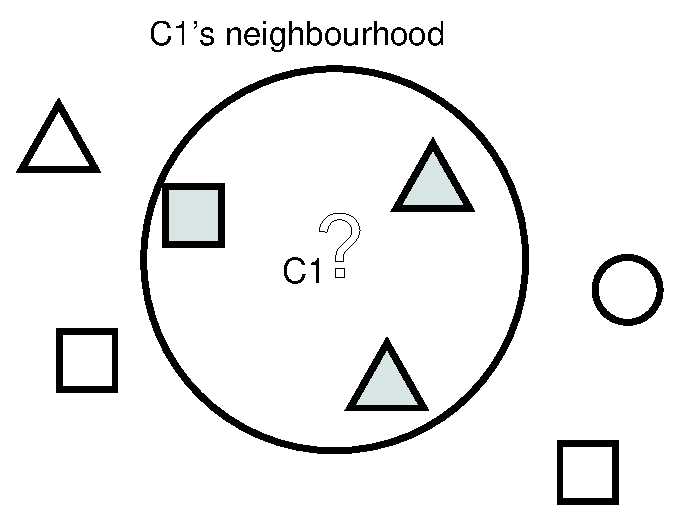
\includegraphics[scale=0.5]{./Drawn/KnnExample}
\caption{Example of a new unlabelled case $C1$ added to a case-base, placed at distances relative to the existing cases in the case-base. At $k=3$, and KNN used, the shaded cases are retrieved as the 3-nearest neighbours. Assuming majority voting, it is classified a triangle.}
\label{fig:knnexample}
\end{figure}

In the example presented in Figure \ref{fig:knnexample}, the shaded cases are retrieved as the nearest neighbours of the new unlabelled case $C1$. 

\subsection{Performing the Classification}

How the unlabelled case gets classified based on the retrieved nearest-neighbours depends on the voting method used, for example:
\begin{itemize}
	\item In majority voting, the most frequent label of the nearest neighbours is used. In the example, two vote `triangle', and one votes `square'. `Triangle' is the more frequent label of the retrieved neighbours, so it is classified `triangle'.
	\item In distance weighted voting, votes are weighted based on the distance between the source of the label and new unlabelled case. Closer neighbours thus get a larger proportion of the vote than far-off neighbours.
\end{itemize}

Having k greater than one has the benefit of trying to minimize the effect of noise in the dataset. Using distance weighted voting as opposed to majority voting also shares this characteristic. 


\section{Getting Labelled Training Data}

To perform classification using KNN (or any other type of machine learning based classification), there is an unavoidable need for labelled training data to initially train the system. Inevitably, how one goes about generating that labelled training data becomes a concern.

In general, the entity which the system may consult if it wishes to determine the true label for a case is termed the \emph{oracle}.

While often, the oracle is a human expert familiar with the domain in question, the oracle may be any type of entity for which there is some expense\footnote{Here, we use the word `expense' in its broadest possible meaning. It may be financially expensive, computationally expensive, or simply take an exceedingly long time to run. In any event, `expense' refers to some undesirable operation for which we want to minimize the number of calls.} in using to determine a label. 

There is a limit to how much data we can ask the oracle to label. If a human expert is needed, this human factor in itself limits the quantity of data which can be labelled. The financial cost might be significant, and the availability of such an expert can also be a limiting factor. As a result of all this, the question of which data is worthwhile labelling comes up.

\section{Active Learning}
The key concept of active learning is that a machine learning program has a say in its own learning process, by being capable of choosing the data from which it learns. 

Not all data is of equal benefit in labelling if it's at the expense of not labelling some other data. We may already have sufficient data for one area of the domain, and be relatively confident in our classifications for that area, but might have very little for some other part of the domain. Given that we can only label so much, it would be preferable, for example, to explore the more unknown part of the domain.

The term \emph{selection strategy} is used to denote the algorithmic approach taken to determine which unlabelled cases to query against the oracle for their true labels, and subsequently put in the case-base with their labels. The \emph{stopping condition} of the system is the point at which the system must stop consulting the oracle.

\section{Active Learning Application Domains}

There are many real-world domains in which a large quantity of unlabelled data is available, but labelling all of that data is not feasible. 

Often the labelling process is in itself exceedingly slow compared to either the amount of unlabelled data available, or the rate at which new data is being collected. 

\subsection{Recommendation Engines}
In recommendation engines, the user can be thought of as the oracle. It is from user feedback (either implicit or explicit) that the recommendation engine can know if an item was relevant to the user or not. It is likely that there is a vast library from which a recommendation can come, but the quantity of user feedback may be limited.

What is sometimes done in these systems is that the engine includes some results it is relatively certain will be relevant to the user, and others of which it is uncertain, but would like to gain feedback on from the user. Only comparatively few of these uncertain cases can be given to the user for feedback, as doing otherwise would negatively impact the user's experience.

Choosing which uncertain cases to present to the user to maximize the system's competence-gain is therefore an important problem for the system.

\subsection{Medical Data}
Medical data is another area in which active learning is of particular interest and relevance.

Vast quantities of patient data exists, but each patient data instance is unlikely to have results of tests for every possible disease / condition. It is obviously preferable though to detect any illness or condition a person has as soon as possible, so that appropriate measures are taken. It is not feasible however to test each individual for every possible illness.

When building a system to predict illnesses, one would want to minimize the number of physical tests to be carried out on patients for the purpose of training the system. It is in this way that active learning can have a useful role to play.

\subsection{Computer Vision}
Computer Vision is another area in which large quantities of data are available, and easy to generate, but manual labelling is incredibly tedious.

\subsection{Text Classification}
With the proliferation of the internet, and in particular social media, text classification has an increasing number practical applications. The traditional example is that of email spam analysis, but more and more, sentiment analysis is becoming an active area of interest.

Vast quantities of textual data are often available for the target domain, though initial labelling requires human involvement. Active learning can play a potentially very useful role in the process, helping in maximizing the system gain with the minimum amount of data.

\subsection{Voice Analysis}

Speech recognition is one area that can bring immense benefit to users, but for which manual labelling requires expert skills, and is painstakingly slow even with a trained expert's involvement. For such systems, it is highly desirable to reduce the quantity of data that must be manually labelled to bring the system to an acceptable rate.

\section{Types of Active Learning}
\subsection{Stream Based Learning}
In \emph{Stream Based Learning}, the system does not just select at the outset the cases to request labelling by the oracle. Instead, it is presented with a stream of cases, and for each case, it may either itself guess the classification (if it is relatively sure it is correct), or it may defer the decision to the oracle.

\subsection{Query Synthesis}
Although it can cause hassle for a human annotator, another variation is known as \emph{Query Synthesis}, in which the program actually constructs its own unlabelled data instances to present to the oracle (as opposed to the data being actual previously observed).

The program is thus able to actively explore the domain space, as opposed to just waiting for data to try to infer this information.

While unsuitable for many problem areas (in particular text), one could easily see how this model could be useful in the context of scientific experiments. The program may wish to make \emph{guesses} as to what would be useful data to get classified, so that it may further refine its knowledge of the domain.

\citet{Settles2010} points to a good example involving a ``robotic scientist'' as described in \citet{King2009}.

Query Synthesis is not really necessary in traditional pool-based sampling areas - since a large pool of truly observed (and therefore valid) unlabelled examples are present that should be representative of the type and distribution of problems which will be later presented to the system.

\subsection{Pool-Based Sampling}

The facet of active learning we will subsequently consider is known as \emph{pool-based sampling} in other literature \citep{Settles2010}, and is based on the idea that there is a large quantity of unlabelled cases available, but getting labels (which might involve consulting a human expert) is an expensive process, for which it is undesirable to apply to the entire unlabelled set. 

The aim of the system is to choose a subset of these unlabelled cases for which to request a label. These are then used as the system's pool of labelled cases which it will consult in future. The system would like to maximize its classification accuracy for future cases, but resort to asking the oracle external to the system for a minimal number of labels.

\begin{figure}[h!] \centering
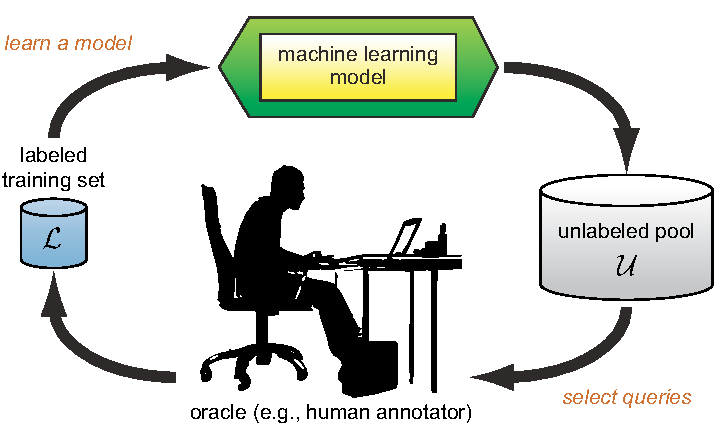
\includegraphics[width=10cm]{./Others/Settles2010PoolBasedImage}
\caption*{Pool-Based Active Learning Cycle Diagram found in \citet{Settles2010}}
\end{figure}

\section{Variations / Related Areas}
Many variations on the concept of active learning exist. The following is intended to give just a small subset of examples, as found in \citet{Settles2010}.

\subsection{Case-Base Maintenance}
\emph{Case-base maintenance} is concerned with the task of how to maintain a case-base. 

Over time, as new cases are added, the case-base size increases. This can have an adverse effect on system performance, thus it can be desirable to have the case-base be as minimal as possible, while maintaining classification accuracy.

Another consideration is that some cases may be adversely affecting the system's classification accuracy. It may be that these cases were initially mislabelled by the oracle, the underlying data was noisy, or it could be that the nature of the domain has changed and that similar cases now actually have a different label. The detection of these cases is therefore an important part to long-running case-based reasoning systems.

Overall, case-base maintenance can be summarised as the process of maintaining a case-base to a desirable level over time. This contrasts to what we will concern ourselves with - how to build a case-base.

\subsection{Seeding in Active Learning}
Many selection strategies have the assumption built in that there are already some cases in the case-base from which they may base their judgements. Thus the issue of how to initially seed the case-base crops up.

In our evaluations and experimentation, we don't attempt to initially seed the case-base - instead starting with an empty case-base. The reasoning for this is twofold: 
\begin{enumerate}
	\item The datasets we use are relatively simplistic, which even with random sampling, converge to a relatively high accuracy even after a small number of samples are added. This would make it very difficult to reasonably compare different selection strategies if seeding were also used. 
	\item Adding seeding would also add another factor for testing, as opposed to primarily testing the variance between different selection strategies.
\end{enumerate}

\subsection{Noisy Oracle}
A \emph{Noisy oracle} relates to the oracle being wrong in its classification some of the time.

In our investigation, we do not deal with this variation at all, assuming a perfect oracle.

\subsection{Labelling Cost Variation}
In many real-world applications, the cost associated with labelling a case can vary from case to case. Some cases can involve much more time to determine a label for than others. In text classification, articles vary in length and complexity. Similarly in video and audio.

In our investigation, we do not deal with case labelling cost variation, instead assuming a fixed cost.

\subsection{Batch Learning}
In practice, it is unlikely that cases would be presented to the oracle one-at-a-time. What is more likely is that batches of cases are presented to the oracle.

In our investigation, we do not perform batch learning - instead presenting cases one at a time to the oracle (equivalent to a batch size of 1).

\section{Report Outline}
\begin{itemize}
	\item Chapter \ref{cha:litreview} will outline various basic selection strategies as found in existing active learning literature, as well as looking at some more complicated strategies.
	\item Chapter \ref{cha:platarch} will give an overview of the platform architecture developed during the course of this project for running and analysing selection strategy experiments.
	\item Chapter \ref{cha:CompetenceModels} will introduce the notion of \emph{Competence Models}, outlining a particular model developed by a researcher from DIT. 
	\item Chapter \ref{cha:compbasedselstrategies} will then proceed to present our attempts at expanding the models, and using them in an active learning selection strategy context.
	\item Chapter \ref{cha:expanalysis} will present the results of the experimental analysis carried out on the basic selection strategies, and our competence based strategies.
	\item Chapter \ref{cha:conclusions} finishes with the conclusions to the project, and potential areas of future work that could follow.
\end{itemize}

\chapter{Literature Review\label{cha:litreview}}
\section{Introduction}
Active learning, and case-based reasoning in general, have massive quantities of research backing them. In this chapter, we will try to give an overview of some basic selection strategies in use in active-learning, along with two examples of recent research efforts to the area.

\section{Common Concepts}
Certain concepts very frequently occur in the active learning literature, so these will be outlined first.

\subsection{Density}
The notion of \emph{density} is extremely common. It simply represents how dense a region is with cases within a large group of cases by means of how close cases are to one another.

Density is usually measured across the entire dataset (i.e. both the unlabelled and labelled pool), as it is of less use to know of dense regions within the labelled dataset when trying to choose cases from the unlabelled data to request a label for\footnote{This, in particular, is true when building the case-base. For case-base maintenance tasks, dense regions within the case-base might indicate redundancy.}. 

The reasoning is that the entire dataset is hopefully representative of real-world cases, of which new cases will appear with similar ranges and distributions. If one selects from a dense region of the unlabelled dataset, it would be hoped that it would cover a large range of input problems.

\begin{samepage}
Even with the commonality of the density notion, there is quite a bit of variance in the literature around how density is actually measured. Two examples of relatively straightforward measures:
\begin{enumerate}
	\item \textbf{Global Density}: The average similarity from a case to every case in the dataset \citep{Xu2007}.
	\item \textbf{Local KNN Based Density}: The average similarity to its k-nearest neighbours in the dataset \citep{Zhu2008}.
\end{enumerate}
\end{samepage}

Density is also sometimes measured for groups as opposed to on a case-by-case basis \citep{Smyth1998}, and often involves the sum of the pair-wise similarities for the cases in the group.

\subsection{Diversity}

\emph{Diversity} (usually also mentioned with density) is another common measure used. It simply represents how different a case is compared to other cases in a group.

In contrast to density, diversity is usually not measured across the entire dataset, but instead just across the actual case-base\footnote{Again, this might be different when one is dealing with case-base maintenance.}. The reasoning for this is that it would be beneficial to select new cases that are diverse from what is already present in the case-base, in hopes that a larger range of the domain may be solved as a result. 

A relatively common metric for the diversity of a case is the similarity to that case's nearest neighbour within the group in question.

\subsection{Solves / Classifies / Contributes}
When it comes to analysing an individual case, often the notion of the other cases that the individual case can somehow classify comes into question. In the context of KNN classification though, an individual case will not be able to classify another case on its own, instead somehow only possibly contributing to another case's classification. This leaves room for different definitions of what one means when they consider a case capable of solving another case. 

\citet{BridgeUpcoming} highlights the interesting point that there are subtle but definitely significant differences to what different researchers mean when they use the term solves. Often, the term seems to be glossed over quickly in literature due to its apparent obviousness, but is still often core to the algorithms presented.

\section{Basic Selection Strategies}
\subsection{Random Sampling}
\emph{Random sampling} is probably the most basic selection strategy. It simply selects cases at random from the unlabelled set. Even with its simplicity, it has the benefit of resulting in a moderately representative sampling of the domain\footnote{This is assuming that the unlabelled cases are a representative sampling of the real world domain - which we usually assume that they are.} if a sufficient number of instances are chosen.

It is often used as one of a group of baseline strategies against which other strategies are compared.

\subsection{Uncertainty Sampling}
\emph{Uncertainty sampling} \citep{Lewis1994} selects cases that a classifier trained on the case-base is most uncertain about (or said another way - is least certain about). Assuming the classifier can generate a probability for each label when provided with a new unlabelled case, the maximum of these for a case can be said to be the \emph{certainty} with which the classifier can classify that case. Picking the minimum of these gives the least certain instance. Uncertainty sampling can thus be defined as, for each unlabelled case, calculating the probability of the most likely label (i.e. the label with the highest probability), and choosing the case with the smallest value to sample.

The rough intuition is that by selecting cases that the classifier is least certain about, you are making the biggest impact on the system by trying to ensure that there won't be new unseen instances that the classifier will be so uncertain of.

The benefit of uncertainty sampling is that it doesn't select redundant cases, since whatever it selects is the one that it is least capable of classifying with its current case-base. The downside is that it is very prone to querying outliers, since it does not consider information such as the density of the region from which the case comes.

Uncertainty sampling, like random sampling, is very commonly used as a baseline when evaluating new algorithms.

\subsection{Uncertainty with Density}
As discussed in the previous section, uncertainty sampling has the serious downfall of being prone to querying outliers, since it does not consider the regions surrounding the cases it selects.

A very straightforward attempt at solving this issue is by incorporating density information also, giving an additional weighting to the uncertainty measures based on how dense a region the case in question comes from. Uncertain cases from dense regions thus become more favourable than uncertain cases from very sparse regions (outliers).

One example of combining uncertainty with density can be found in \citet{Zhu2008}, though it uses an uncertainty measure based on Entropy as opposed to pure uncertainty alone.

\subsection{Margin Sampling}

\emph{Margin sampling} tries to account for a shortcoming in pure uncertainty sampling for multi-label classification in that it only considers information about the most probable label, essentially throwing away the information about the other labels.

Margin sampling looks at the difference between the probability of the most probable label, and the second most probable label. The intuition is that if there is a large difference between the two, the classifier must be relatively certain. On the other hand, if there is very little difference, then with relatively little change, the classifier might have picked a different label, and so it really mustn't have been very certain about it.

Margin sampling only makes sense in classification where there are more than two possible label values. In binary classification, Margin sampling gives an identical strategy to uncertainty sampling.

\subsection{Diversity Only}
In \emph{diversity only} sampling, the system selects cases that are as far away as possible from everything else in the case-base. This can result in an understandably diverse case-base, but is very prone to querying outliers like uncertainty sampling.

This motivates many authors to try and incorporate density information with diversity. One such attempt is described next.

\section{Rong Hu's Work on EGAL: Exploration Guided Active Learning}
\subsection{Introduction}
Many selection strategies have firm dependencies on a type of classifier confidence score (what Hu terms \emph{exploitation}), while also incorporating measures such as density and diversity (what Hu terms \emph{exploration}).

Hu, in her work on EGAL \citep{Hu2011}, experiments with developing an exploration only strategy by combining measures of density and diversity\footnote{Rong Hu recently completed her PHD Thesis on ``Active Learning for Text Classification'' in D.I.T. with Dr. Sarah Jane Delaney as one of her supervisors \citep{Hu2011}. In her thesis, she covers a broad range of topics, but of particular interest to us is her work on ``EGAL'', and also on using aggregate confidence measures.}.

While some of the formula specifics feel slightly odd, the overall attempt at using an exploration only strategy is pretty interesting. 

\subsection{Hu's Density / Diversity Measures}

\subsubsection{Density}
Hu defines a case's \emph{density} as the sum of similarities within a case's neighbourhood.
\[
density(x_{i})=\underset{x_{r}\in N_{i}}{\sum}sim(x_{i},x_{r})
\]

The neighbourhood $N$ of a case $x_{i}$ within the entire dataset $D$ she defines as:
\[
N(x_{i})=\left\{ x_{r}\in D\mid sim(x_{i},x_{r})\geq\alpha\right\} 
\]

$\alpha=\mu-0.5\times\delta$ where $\mu$ is the mean, and $\delta$ is the standard deviation of the similarities. This value for $\alpha$ is somewhat arbitrary, in that it just seemed to work well in Hu's experiments.

Of particular note is that the density measure is calculated across the entire dataset $D$ (i.e. unlabelled and labelled). 

\subsubsection{Diversity}

Diversity measures how different a case is from everything already in the case-base (all the labelled cases $L$).

\[
diversity(x_{i})=\frac{1.0}{max_{x_{r}\in L}sim(x_{i},x_{r})}
\]

In this formula, similarity is inverted because distance is the inverse of similarity. So diversity is really the distance to the nearest neighbour in the labelled set.

\subsection{The EGAL Strategy}

\subsubsection{Overview}
Hu's approach is to build a candidate set of cases from the unlabelled set which one might want to add to the case-base. This candidate set is based roughly on the cases that are furthest away from all the cases in the case-base (i.e. the most diverse cases). From these candidates, one then chooses cases that are from dense regions of the case space.

Hu allows for the balance between the effect of density and diversity to be controlled through a ``balancing factor''.
 % Fight to get heading next to algorithm

\begin{samepage}

\subsubsection{The EGAL Algorithm} 

\begin{figure}[h!] \centering
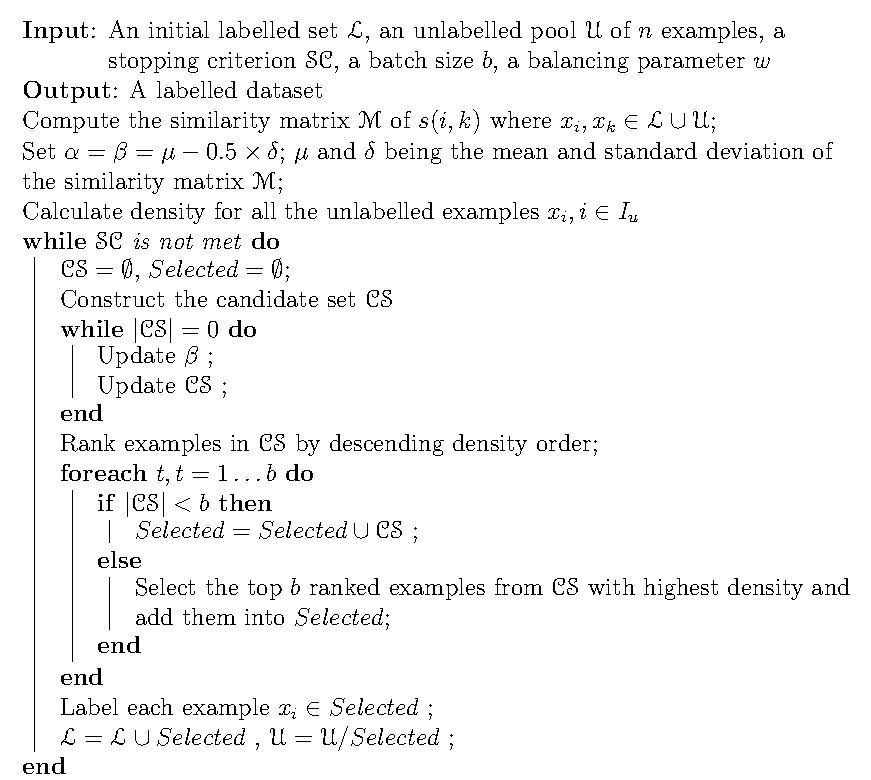
\includegraphics[scale=0.75]{./Others/Hu2011EgalAlgorithm}
\caption*{Hu's Algorithm for the EGAL Selection Strategy}
\end{figure}

\end{samepage}

\subsubsection{Candidate Set}
\[
CS=\left\{ x_{i}\in U\mid diversity(x_{i})\geq\frac{1}{\beta}\right\} 
\]

This is presented in a slightly expanded (but equivalent) form in Hu's paper dedicated to EGAL \citep{Hu2010}. Really, $\beta$ represents the maximum similarity allowed to its nearest neighbour. This formula forms the set of cases within the unlabelled set $U$ which do not have any other cases within a distance of $\frac{1}{\beta}$.

\subsubsection{Generating the Max Similarity Sets}

Firstly, for each item in the unlabelled set $U$, the similarity to the \emph{closest} element in the labelled set is calculated and stored\footnote{Diversity is the distance to the closest element. The inverse of distance gives similarity. Thus the inverse of diversity is the similarity of an element to its closest element.}.

\[
S=\left\{ s_{i}=\frac{1}{diversity(x_{i})}\mid x_{i}\in U\right\} 
\]

\subsubsection{Determining $\beta$}
The setting of $\beta$ feels somewhat round-about - but roughly speaking, $\beta$ is set to the similarity value that would cause a certain pre-fixed percentage of the top-most diverse elements to be chosen as the candidate set.

Firstly, a proportioning parameter $w$ controls the proportion of the top-most diverse elements to include in the candidate set. From experimentation, Hu finds that 0.25 gives good results - i.e. selecting a quarter of the most diverse elements as the candidate set.

Because, in the algorithm, similarity values are spoken about instead of proportions, we must find the threshold similarity value ($s_{w}$) that would result in that proportion.

\[
S_{1}=\left\{ s_{i}\in S\mid s_{i}\leq s_{w}\right\} 
\]

\[
S_{2}=\left\{ s_{j}\in S\mid s_{j}>s_{w}\right\} 
\]

\[
\left|S_{1}\right|=\left\lfloor \left(w\times\left|S\right|\right)\right\rfloor +1,\hphantom{}0\leq w\leq 1
\]

$\beta$ is then set to that $s_{w}$ value.

\subsubsection{Algorithm Outline}
\begin{enumerate}
	\item Initially $\beta$ is simply set to $\alpha$, but is updated according to the formula above each time the candidate set becomes empty.
	\item The candidate set is sorted from highest density to lowest density, and items are taken in order until the stopping condition is reached.
\end{enumerate}

\subsubsection{Factor Summaries}
\begin{itemize}
	\item $\beta$ represents the maximum similarity that labelled examples should be from an unlabelled example to be thought of as \emph{diverse}, and thus should be included in the \emph{candidate set}.

	\item $\alpha$ relates to the distance (really similarity) within which to define the neighbourhood of a case for the purpose of calculating the density (total pairwise similarity) of the case. 
	
	This is represented in terms of similarity - the minimum similarity value cases should have to be within the neighbourhood.
	
\end{itemize}

\subsubsection{$w$ as a Density/Diversity Balancing factor}
Hu explains that $w$ is a balancing factor between density and diversity \citep{Hu2010}. 

\begin{itemize}
	\item When $w=0$, a pure diversity-sampling approach occurs. 
	\item When $w=1$, a pure density-sampling approach occurs. 
	\item When $w$ is set to values between $0$ and $1$, a mixture of density and diversity sampling occurs.
\end{itemize}

\subsection{Experimental Results}
In \citet{Hu2011}, Hu finds that $w=0.25$ gives the best results for the datasets she used. 

Hu also finds that the EGAL strategy with $w=0.25$ compares favourably with random sampling, and also beats diversity-only and density-only sampling.

For comparison with other active learning strategies, Hu finds that EGAL performs generally better than the other strategies at the initial stages of the active learning process.

\subsection{Comments}
Even though $w=0$ gives a diversity-only approach, and $w=1$ gives a density-only approach, it is unclear the exact effect of having values in between the $0$ to $1$ range.

The approach of picking a similarity value to achieve that partitioning also feels unnecessarily complicated.

\section{Rong Hu's Work on Aggregating Confidence Measures}
\subsection{Introduction}
Before continuing, confidence probably needs to be initially distinguished from competence. \emph{Confidence} relates to how confident the system is regarding the classification of an unseen instance (e.g. the probability of the most likely label as determined by the classifier), whereas \emph{competence} relates to the overall capability of the system. It is confidence measures that are dealt with here.

In her thesis \citep{Hu2011}, Hu outlines a selection strategy based on using a single confidence measure (essentially, the same as standard uncertainty sampling, but using the confidence measure to determine what the case-base is most uncertain of), but expands on this to present an algorithm which attempts to aggregate multiple confidence measures, to produce an algorithm that performs better than using any one of the confidence measures alone.

\subsection{Model \& Measures}

In \citet{Delany2005}, five confidence measures are proposed. Hu chooses the three of these which she determines experimentally to have the least correlation\footnote{The validity / appropriateness of this approach will not be considered further though - since this particular paper - and the piece of interest to us - is that of aggregating confidence measures. Further descriptions, explanations and justifications of the measures can be found in \citet{Delany2005}}.

For the three, the following metrics are needed:
\begin{itemize} 
	\item $N_{i}(t)$ denotes the ith nearest neighbour of example t.
	\item $NLN_{i}(t)$ denotes the ith nearest like\footnote{\emph{Like} and \emph{unlike} are compared to the case's predicted label by the KNN classifier, since obviously, the actual label of the case is unknown.} neighbour to example t.
	\item $NUN_{i}(t)$ denotes the ith nearest unlike neighbour to example t.
\end{itemize}

\subsubsection{Average NUN Index}

\[
AvgNUNIndex(t,k)=\frac{\sum_{i=1}^{k}IndexOfNUN_{i}(t)}{k}
\]

where:
\begin{itemize}
	\item $IndexOfNUN_{i}(t)$ is the index of the ith nearest unlike neighbour of target example t, the index being the ordinal ranking of the example in the list of NNs
\end{itemize}

This represents the average index of the first k unlike neighbours in the case's sorted nearest neighbour list. Intuitively, a larger average index is preferable, as this somewhat indicates that there wasn't much uncertainty, when the closer neighbours were voting for the predicted label.
\vspace{10pt}

\begin{samepage}

\subsubsection{Similarity Ratio}
\[
SimRatio(t,k)=\frac{\sum_{i=1}^{k}Sim(t,NLN_{i}(t))+\epsilon}{\sum_{i=1}^{k}Sim(t,NUN_{i}(t))+\epsilon}
\]

where:
\begin{itemize}
	\item $Sim(a, b)$ is the similarity between examples $a$ and $b$ 
	\item $\epsilon$ is a smoothing value to allow for situations where an example may have no NLNs or NUNs ($\epsilon$ = 0.0001 is used in all of her evaluations). Top and bottom have this value to give a ratio of 1 when there are no NLNs or NUNs.
\end{itemize}

This represents the ratio of the similarity values between a case's k-nearest like neighbours, and its k-nearest unlike neighbours. Intuitively, a higher ratio is better, as this would indicate that the classifier should be certain about its classification, since the cases with the same label as the predicted label are relatively a lot closer than the ones of a different label.

\end{samepage}

\subsubsection{Similarity Ratio Within K}
\[
SimRatioK(t,k)=\frac{\sum_{i=1}^{k}Sim(t,NN_{i}(t))\delta_{t,NN_{i}(t)}}{\epsilon+\sum_{i=1}^{k}Sim(t,NN_{i}(t))(1-\delta_{t,NN_{i}(t)})}
\]

where:
\begin{itemize}
	\item $Sim(a, b)$ is as above, 
	\item $\delta_{a, b}$ is Kronecker's delta where $\delta_{a, b}=1$ if the label of $a$ is the same as the label of $b$ and $0$ otherwise. 
	\item $\epsilon$ is a smoothing value to allow for situations where an example may have no NUNs ($\epsilon = 0.0001$ is used)\footnote{It's unclear the reason for the inconsistency between the use of $\epsilon$ on the bottom only in $SimRatioK$, but on top and bottom in $SimRatio$.}.
\end{itemize}

This measure is similar to the $SimRatio$ measure, except that instead of considering the k-nearest like neighbours, and the k-nearest unlike neighbours, it just considers the like and unlike neighbours within the first k-nearest neighbours (be they like, or unlike).

\subsection{Combining the Confidence Measures}

\subsubsection{Overview}
Firstly, in a machine learning fashion, the threshold values are determined for each measure for each label that indicate confidence for that label. These predicted values are then used in assembling a non-confident set, from which elements are selected in a least-confident-first style. This selection happens in `batches', after which the algorithm is re-initialized for the next batch. This is repeated until the stopping condition is met.

\begin{figure}[h!] 
\subsubsection{The ACMS Algorithm}
\centering
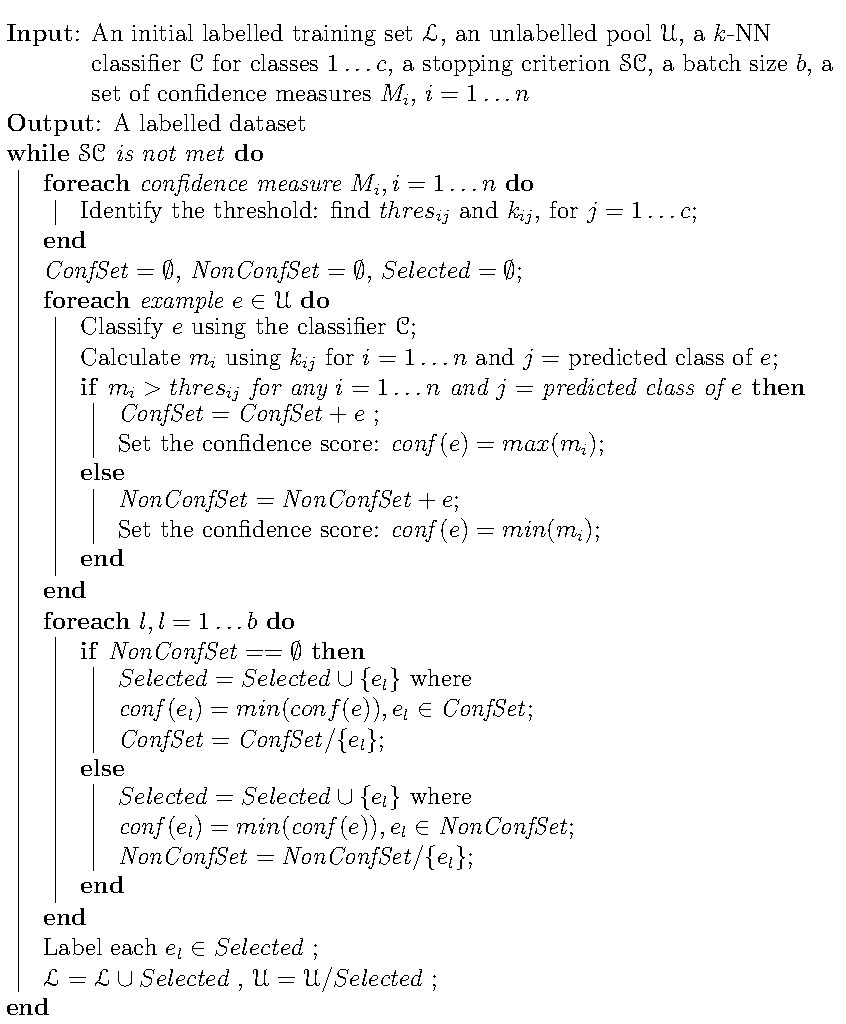
\includegraphics[scale=0.7]{./Others/Hu2011AggregrateAlgorithm}
\caption*{Hu's Algorithm for the Aggregated Confidence Measures Selection Strategy}
\end{figure}

\subsubsection{Initializing the Case-base}
Before the main algorithm which combines the confidence measures is initiated, the case-base is initially seeded with a deterministic variation on Furthest-First Initialization, as presented in \citet{Greene2007}.

\subsubsection{Confidence Measure Threshold Initialization}
For \textbf{each} measure, the confidence threshold needs to be identified for \textbf{each} label.

For each measure, predictions with confidence values higher than the predicted label's threshold are considered confident for that measure, while those with values below are considered non-confident for that measure.

Details surrounding how exactly these thresholds are set can be found in \citet{Delany2005}, but roughly, values are chosen on a per-dataset basis through experimentation, with a threshold calculated for each measure for each label (i.e. cross product style) that maximizes confidence-accuracy while keeping False Positives to zero. This is done because of the boolean nature on which the measures apply, but in the context of classification where there might be more than two labels. 

\subsubsection{Operation}
The algorithm essentially operates on repeatedly building two sets from the unlabelled data - the confident set, and the non-confident set.

The confident set is composed of cases for which any of their confidence measures exceeded the measure's confidence threshold. The \emph{score} associated with each case is the maximum of all the confidence measures for that case.

The non-confident set is composed of cases which do not appear in the confident set, but the \emph{score} associated with each case is the minimum of all the confidence measures for that case. 

This min-max combination was chosen as it performed the best in Hu's preliminary experiments when she considered multiple variations\footnote{I question the validity of this approach. For discussion, see Section \ref{sec:hu2comments}.}. Measures for each case ``are normalized using statistical normalization after performing a log transformation to correct those with skewed distributions'' \citep{Hu2011}.

After the confident and non-confident sets are built, selection begins. First elements in the non-confident set are selected, and once it is expended, elements from the confident set are selected. Selection occurs from each of the sets in a lowest-score-first order. A batch size, which is an input to the algorithm, indicates how many should be selected in this \emph{batch}, before restarting the entire process, and beginning the selection of a new batch from the start again.

\subsection{Experiment Results}
Hu finds that using the ACMS strategy performs marginally better than using any one of the confidence measures alone. She also finds that the strategy, with Delany's measures, performs better than an uncertainty sampling based selection strategy.


\subsection{Comments\label{sec:hu2comments}}
I am unconvinced about the validity of the min-max style of aggregating the confidence measures.

The paper and thesis section seem rather unspecific about how the measures are normalized. I'm guessing there are broadly two possibilities :

\begin{enumerate}
	\item \textbf{Measure Threshold Normalization}
	
	In this possibility, measures would be normalized so that their thresholds would be the same.
	
	I don't think this was the method used. If the thresholds alone were normalized, the measure ranges' maximum possible values would be different. As a result the maximum measure scores would definitely not be directly comparable.
	
	\item \textbf{Measure Range Normalization}
	
	In this possibility, the range of values over which the measure falls is normalized - giving the same minimum and maximum value possible for each measure. I don't think the measure threshold could then also be normalized, leading to different measures very likely having different thresholds. 
	
	If any measure passes its respective threshold though, the maximum measure's value is chosen as the case's score, but this score may have nothing to do with the measure that actually caused the case to fail to be classed as confident. Scores are subsequently compared with other scores.
	
	\begin{samepage}
	For examle, for a given label, 
	\begin{itemize}
		\item $thres(M1) = 0.8$
		\item $thres(M2) = 0.2$
	\end{itemize}
	and for a given case $case_{1}$ for that label:
	\begin{itemize}
		\item $m1 = 0.7$
		\item $m2 = 0.3$
	\end{itemize}  
	\end{samepage}
	Because $m2 > thres(M2)$, the case will be put in the confident set, and as such, the maximum of the measures will be taken: $m1=0.7$. Really though the confidence measure that passed the threshold was $m2$ with a value of $0.3$.
	
	Now, imagine a different case $case_{2}$, but for the same label as above\footnote{The reason I'm specifying the same label is just to emphasize that the same thresholds apply. If it were a different label, different thresholds may apply - since thresholds are on a label-by-label basis - thus adding unnecessary complication to the example.}:
	\begin{itemize}
		\item $m1 = 0.1$
		\item $m2 = 0.6$
	\end{itemize}
	Again, because $m2 > thres(M2)$, the case will be put in the confident set, but the maximum measure will be $m2 = 0.6$. 
	
	$case_{1}$ (with a score of $0.7$) will be treated as more \emph{confident} than $case_{2}$ (which has a score of $0.6$), even though $case_{2}$ was actually more confident than $case_{1}$ in the measure that actually caused it to be confident ($M2$).
	
\end{enumerate}

Whichever was the actual methodology, both seem flawed. The underlying fact remains that the different confidence measures aren't directly comparable, and the relatively simplistic manner in which the presented aggregation strategy deals with them - simply taking the maximum of all of them when any one is confident - does not appear to take this into account. Similarly with taking the minimum for the non-confident set.

It's possible that there was some advanced maths way, of which I am unaware, to do the normalization which might hope to account for both range and threshold normalization, but I can't see how it could change the fact that a score is being assigned based on possibly a different confidence measure than the one which actually achieved confidence.

As a result of the above, we decided not to proceed with using Hu's aggregation strategy.

\section{Conclusions}
From reviewing a sampling of current active learning literature, it appears that no one to date has used purely competence based selection strategies. It is this gap that we wish to tackle. 

Even with the abundance of active learning research, there does not appear to be any single widely used platform for selection strategy research. In the next chapter, we present the research platform we developed for the purpose of our experimentation and investigation into competence based selection strategies.

\chapter{Platform Architecture\label{cha:platarch}}
\section{Overview}
\subsection{Purpose}
The purpose of the system is to allow evaluation of and comparison between different selection strategies in a pool-based active learning context.

It achieves this by executing each of the selection strategies on several datasets from an initially empty case-base. At each selection in the selection strategy, it runs a KNN based classifier on the case-base, evaluating its capability to correctly classify the instances in a test set.

\subsection{Technologies}
Weka \citep{prog:weka}, a Java based machine learning framework, was initially briefly investigated, but due to my familiarity with Python, Orange \citep{prog:orange} was used as the core machine learning component. It provided useful facilities to quickly get a basic evaluation platform up and running. As the platform progressed, most Orange dependencies were removed in favour of custom implementations due to the need for greater control, and a memory-management related bug which existed in Orange with regards its Python bindings for its C++ backend. Orange was subsequently just used for data loading, and distance computations.

For plotting, matplotlib \citep{prog:matplotlib} was initially used, but due to its very non-pythonic interface, we changed to using PyX \citep{prog:pyx}, which also provided much better support for \LaTeX{} style file formats.

Towards the end of the project, a basic python map-reduce framework `mincemeat' \citep{prog:mincemeat} was integrated into the platform to allow cluster-style operation.

\begin{figure}[h!]
\subsection{High Level Data Flow Diagram}
 \centering
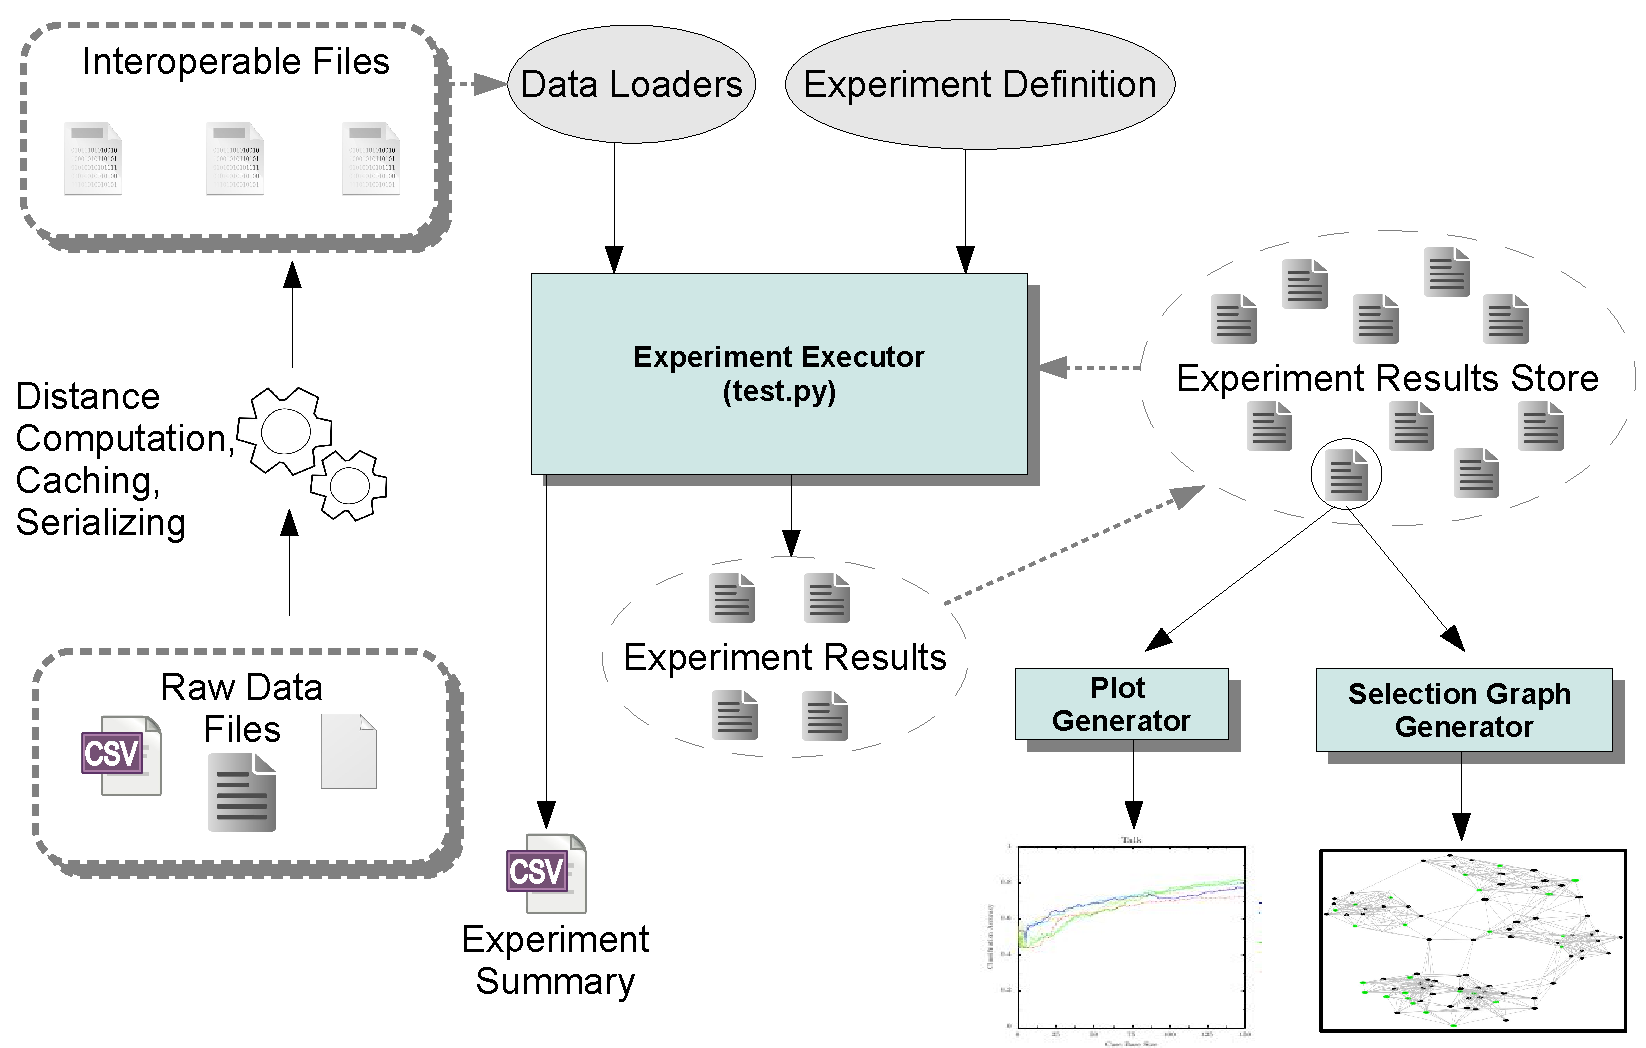
\includegraphics[width=10cm]{./Drawn/DataFlowDiagram}
\end{figure}

\section{Inputs}
\subsection{Data Files}
Data files provide a table of instances, each instance consisting of attribute values and a label. Orange provides support for loading many common formats, and also is capable of performing distance computation between cases based on their attributes.

For ease, Orange was used to perform initial data loading, and distance computation between cases. The instances, and their pair-wise distances, were then serialized to a new data file to allow running on platforms (and runtimes) for which Orange wasn't present.

\subsubsection{Orange Supported}
Orange's primary data format is that of tabular, delimited text - such as CSV or TSV. Optionally, markup can be placed in the header rows of these files to help Orange know of the properties of each of the attributes - e.g. if the attribute represents the label for the case, if the attribute is discrete or continuous, etc., but Orange is surprisingly good at figuring most of it out on its own - occasionally just needing slight nudging in the right direction.

Orange also supports some of the formats commonly used in other Machine Learning platforms - e.g. ARFF (as found in Weka) and correctly formatted .names, .data file pairs as sometimes found in the UCI Machine Learning Repository \citep{web:uci}\footnote{It should be noted that the majority of .data/.name pairs are not in the strict format necessary, thus some prior manipulation of the files present there may be needed to load them with Orange.}.

\subsubsection{Custom Pre-computed Distance Format}

The $n \times n$ distance matrix for a dataset can really be stored in a symmetrical matrix\footnote{This is assuming that the distance function is in fact symmetric, i.e. $d(a, b)\equiv d(b, a)$. In our distance function, this property does hold.}. Thus, when storing the distances for all pairs in the file, the space may essentially be halved by storing only one half of the $n \times n$ matrix\footnote{Technically, the distances between cases and themselves need not be stored, because by definition the distance between a case and itself will be 0. Though this minor optimization is not performed in my code}.

\medskip

\begin{tabular}{ c c c c c c }
	Case ID & \multicolumn{5}{c}{Distances} \\
	0 & $d(i_{0},i_{0})$ &  &  &  & \\
	1 & $d(i_{1},i_{0})$ & $d(i_{1},i_{1})$ &  &  &  \\
	2 & $d(i_{2},i_{0})$ & $d(i_{2},i_{1})$ & $d(i_{2},i_{2})$ &  & \\ 
	... & ... & ... & ... & ... & \\ 
	j & $d(i_{j},i_{0})$ & $d(i_{j},i_{1})$ & $d(i_{j},i_{2})$ & ... & $d(i_{j},i_{j})$ \\ 
\end{tabular}

\medskip

In addition to storing the distances, the label and a textual human-readable payload/case descriptor is also stored along with each case ID.

\paragraph{CSV}
The initial file type used for storing the precomputed distances along with the data was CSV (Comma Separated Values). The first line contains a header row. Subsequent lines contain the data rows. The first data row represents case ID 0, the second represents case ID 1, and so on. Each data row is organized as follows, where distances are stored in a half $n \times n$ matrix as described above:
\medskip

\begin{tabular}{ |c| |c| |c| }
	Textual Case Description & Case Label & Distances \\
\end{tabular}

\medskip

These files may also be gzipped - resulting in an extension .csv.gz, and this will be automatically uncompressed by the platform. The reason support for compression was added was due to the large file-sizes that resulted from the textual representation of the distances.

CSV was chosen due to it being quite trivial to produce irrespective of the programming language. It also allowed for easy debugging, and would potentially allow other machine learning systems to be used for distance computation.

\paragraph{Google's Protocol Buffers \citep{prog:protocolbuffers}}

Google's blurb for Protocol Buffers is ``think XML, but smaller, faster, and simpler'' \citep{prog:protocolbuffers}. It is a binary format for which a proxy can be automatically generated for Python (among many other languages). It is used as the preferred method of loading data with precomputed distances in the presented platform, due to its compact representation, and efficient loading.

These files store essentially the same information in a similar method as the CSV style presented above. The devised protocol specification is as follows:
 
\begin{code}
message Case\{
    optional string payload = 1;
    required string label = 2;
\}

message PrecomputedDistanceData\{
  optional string data_set_name = 1;
  optional string data_set_description = 2;
  
  message Entry \{
    required Case case = 1;
    repeated double distances = 2 [packed=true];
  \}
  
  repeated Entry entry = 3;
\}
\end{code}


Most bits to the protocol are self explanatory. The number following each field is simply the field ID. In the Protocol Buffers specification, each field must have an integer ID, with each ID unique within its local namespace. The ``[packed=true]'' section is simply an optimization that allows the Protocol Buffers engine store the repeated numeric values in as compact a representation as it can.

\subsection{Experiment Definitions}
The definitions for the experiments to run need to be provided to the platform. Each experiment consists of data\footnote{ The data is provided as (training set, test set) pairs to allow for Cross-Validation, etc.} and the selection strategies to run on the data.

\subsection{Existing Results}
Existing results for selection strategies executed on the Data may also optionally be provided with the experiment. When the experiment is being executed, if it can find the results for a selection strategy within the provided existing results, these will be used as opposed to re-running that selection strategy again.

This allows for new selection strategies to be added and run, without re-computing previous strategies, but still having all outputs, such as plots, include the previous strategies' results.

It also allows for the graphs, etc. to be generated separately from the main experiment running\footnote{This can be useful, as then all the plotting/graphing dependencies need not be installed on all machines/platforms the experiment is being executed on.}, and due to ease of re-combining existing results, allows the experiment to be split, and different selection strategies be evaluated on separate machines concurrently.

\section{Experiment Execution}
\subsection{Selection Strategy Evaluation}
\subsubsection{Overview}
In selection strategy evaluation, the purpose is to execute a selection strategy against unlabelled training data\footnote{It's not really unlabelled - it's just from the perspective of the selection strategy it's unlabelled.}, to choose cases from the set and put them in the case-base with their labels until the stopping condition is satisfied.

After each selection, a KNN based classifier is given the case-base as training data, and run on the test set, with the resulting classification accuracy recorded.

The motivation is to judge how good each selection strategy is at selecting cases to maximize the ability of the case-base to classify unseen instances.

\subsubsection{Selection Strategy}

A selection strategy in the platform is responsible for selecting cases to consult the oracle for, given knowledge of what is already in the case-base, and a pool of unlabelled cases to select from.

\subsubsection{KNN Classifier}
A k-nearest neighbours based classifier is used in the evaluation, with 
\begin{itemize}
	\item $k=5$
	\item Distance as defined in the dataset loaded\footnote {For tabular data, Euclidean distance was used - this functionality provided entirely by Orange. For textual data, TF-IDF vectors were generated on the raw non-stemmed documents, and the cosine similarity between documents' TF-IDF vectors computed. This functionality was provided through a combination of SciKit-Learn, and NumPy. The similarities were subtracted from 1 to give the distances.}.
	\item Distance Weighted Voting. The distance function used is:
	
	\[
	\frac{1}{distance^{2}+1}
	\]
	
	where $distance$ is normalized between $0$ and $1$.
	
	
\end{itemize}

\subsubsection{Cross Validation}

10-Fold Cross Validation is used for training/testing against the data. Initially Orange was used to provide stratified folds. Later, when we modified our decision and lessened our reliance on Orange, a simplistic non-stratified implementation was adapted from the SciKit Learn library \citep{prog:sklearn}.

Many walkthroughs of K-Fold Cross Validation exist online \citep{web:kfolddemo}, but the basic approach is to split the data into k sets\footnote{This is an entirely different k than the one in the KNN classifier}, followed by iteratively choosing one of the sets as the test set, and the union of the remaining sets as the training set. The results of the k tests are averaged to produce a single result.

\subsubsection{Basic Evaluation Algorithm}
\nopagebreak[4]
\begin{code}
let result_sets = \{\}
for each (training_set, test_set) in the CV Sets:
  let unlabelled_set = training_set
  let case_base = \{\}, result_set = \{\}
  while the stopping criteria is not met:
    let selections = select cases from unlabelled_set using 
                     the selection strategy.
    ask oracle for labels for all of selections
    remove selections from unlabelled_set
    add selections to case_base with their labels
    let result = Result from testing the classifier
                 built using case_base on test_set
    add result to result_set
  add result_set to result_sets
\end{code}

\subsection{Experiment Outcome Representation}
\subsubsection{Result}
An individual \emph{Result} consists of:
\begin{itemize}
	\item Size of the case-base
	\item Classification accuracy of the case-base
	\item Selections from the selection strategy that were just added.
\end{itemize}

\subsubsection{Result Set}
A \emph{Result Set} is a collection of Results. For convenience and completeness, a Result Set also has knowledge of the training set and the test set that was used in generating the contained Results.

\subsubsection{Multi Result Set}
A \emph{Multi Result Set} is a collection of Result Sets, which provides averaging of Results grouped by case-base size. This is necessitated by the fact that we are performing cross validation. Instead of one Result Set being produced for an experiment, k are produced where k is the number of folds of cross validation being performed.

The Multi Result Set provides an encapsulation of these k cross validation results by allowing them to subsequently act as a standard Result Set based on the averaged results, except obviously, the Training Data, Test Data and Selections fields for this will be blank - since these entities can't really be averaged meaningfully.

\subsection{Summarising The Results}
\subsubsection{Learning Curve}\label{sec:multiresultset}
A commonly presented representation of selection strategy evaluation is the \emph{learning curve} - a plot of classification accuracy vs case-base size.

\subsubsection{Area Under the Learning Curve}
A metric to summarise the progression, and allow for comparison among different selection strategies against the same dataset and same starting and finishing case-base size is \emph{AULC (Area Under the Learning Curve}). As can be expected, this is simply the area under the learning curve. Result Set objects have the inbuilt capability of computing the AULC value for their contained Results.

\subsection{Cluster-Based Execution}
Due to the enormity of data processing involved, as a slight deviation towards the end, cluster based platform execution was implemented. Unused lab machines were used to perform approximately two thousand compute hours worth of experiments. At peak, the platform was executing slave processes concurrently on just over 200 machines - 400 processor cores. 

\subsubsection{Map Reduce Framework: Mincemeat}
Mincemeat \citep{prog:mincemeat} is a relatively simple implementation of a Map Reduce framework, written in pure Python. While not as fully featured as other more developed frameworks, it was chosen for its simplicity, which allowed easy understanding, modification, and portability, having no dependencies other than Python.

\subsubsection{Work Unit Definition}
Independent work units are first computed by the platform before providing to the map reduce framework. They represent the smallest unit of work that the platform can meaningfully execute.

\begin{code}[numbers=none,frame=none] 
Work Unit:
  Dataset Name
  Variation Name
  Experiment Name
  Data Definitions Name
  Raw Results File
  Total Num Folds
  Fold Number
\end{code}

\subsubsection{Map / Reduce Operations}

The map operation takes a work unit, runs the sub-experiment specified, and returns the raw results for the specified fold.

The reduce operation takes the results for all of the folds of a single experiment variation on a dataset, and merges them to a Multi Result Set, which is then written out to disk.

\subsubsection{Handling Failures}

In the given environment, failures of nodes and jobs was an inevitability. Computers are continuously being turned off / rebooted, and sometimes other tasks can be running on a machine meaning that a mapping operation being run on that machine would be essentially non-terminating.

Thankfully, mincemeat provided sufficient handling for these circumstances. Any time spare capacity is available, it re-sends unfinished maps to use the capacity.

Failure of the `master' was less well handled by the framework. Maps were carried out first until all were successfully completed, followed by the reduces. If the master died, or a bug occurred, all the completed maps would be lost. The framework was modified to allow early reduction of a reduce group, if the user could give a guarantee that no more values for the reduce group would be produced in any of the remaining map operations.

\subsubsection{Execution Environment}
One problem with using the college lab computers was the very dated Ubuntu installation present on the machines. To get around this, virtualenv \citep{prog:virtualenv} was used to set up an isolated Python environment in a network-hosted home directory. The `.bashrc' file was then updated to correctly activate this environment upon login.

To allow for promptless operation, public/private key pairs were generated and installed to the executing user's SSH environment. On the master node, given that root access was available, the SSH configuration was changed to automatically accept without prompt previously unseen public keys.

SSH access was then used to initiate a slave process on each available machine, after the master server on a dedicated machine was started. A script was written to first check if a slave process was currently active on the machine, and to only initiate a new one if no other was executing. This allowed ``topping up'' of machines as more became available. The status of the script was then provided back to the master for the accounting purpose of tracking the quantity of active machines.

\section{Outputs}

\subsection{Raw Selection Strategy Results}
The primary and non-optional outputs of the platform are the raw selection strategy results for all the provided datasets. From these, the other outputs can be calculated. It is also these raw results which can be provided to another run of an experiment so that they need not be re-computed if they are needed by the experiment. 

For space efficiency, and ease of manipulation, each set of selection strategy results for a dataset are stored in a compressed archive.

These Raw Results represent the serialized form of a Multi Result Set. When the Raw Results are provided to the program, they are deserialized to Multi Result Sets.

\subsubsection{Individual Cross Validation Results}
For each dataset and subsequently for each selection strategy - the evaluation on each selection strategy is carried out multiple times due to the k-fold cross validation methodology used. As such, there will be k different sets of results. 

Within the compressed selection strategy results archive, these are labelled 0.csv, 1.csv, etc. with each corresponding to the fold number in the cross validation splits of the dataset.

Each csv contains essentially 3 items:

\begin{enumerate}
	\item Results for various case-base sizes, with each Result instance denoted with:
		\begin{itemize}
			\item The case-base size
			\item The classification accuracy
			\item The list of selections that were made by the selection strategy just prior to this test.
		\end{itemize}
	\item The training set used for this fold of cross validation
	\item The test set used for this fold of cross validation
\end{enumerate}

\subsubsection{Summary Results}
Summary Results are also saved\footnote{Technically, these Summary Results are unnecessary, as they can simply be recomputed using the raw individual Cross Validation Results. They are simply there for user ease.}, and are similar to the CSV style of Raw Cross Validation Results except that they do not contain lists of selections, or the test set or training set. They are saved to a file named ``summary.csv''.

\subsection{Learning Curve Plots}
PyX \citep{prog:pyx} is used to generate a PDF file of plots of the learning curves for all of the selection strategies\footnote{Initially - matplotlib \citep{prog:matplotlib} was used to generate the graphs - but its interface was somewhat messy and non-pythonic.}. One PDF is generated for each dataset.

\subsection{Selection Graphs\label{sec:selectiongraphs}}
We also generate a visualisation of the case-base that each selection strategy produces. The distance matrix for the entire dataset is used to generate a spring-graph of all the cases, where each case (represented by a node in the graph) has an edge to a small proportion of its nearest neighbours, with a force proportional to the distance. Graphviz \citep{prog:graphviz} was used to perform this graph generation, with PyGraphviz \citep{prog:pygraphviz} as the interface from Python.

Cases which a given selection strategy chooses are highlighted at each selection iteration. These are then output to a PDF file, with each page representing an iteration in the selection strategy. Examples of the final state of these, after the stopping condition has been reached, can be seen in Figure \ref{fig:selectiongraphexample}.

Because selections can't really be averaged across the different folds in cross validation, a PDF file is generated for each cross validation fold. White nodes represent test cases, grey nodes represent unlabelled cases, and black nodes represent cases selected by the selection strategy.

Due to the flattening of varying dimensionality datasets, the usefulness of these graphs vary widely depending on the datasets used, so it is not beneficial for all datasets.


\begin{figure}[ht]
\centering
\subfigure[Selections graph for `Sparsity Minimization' on `zoo' dataset]{
\includegraphics[width=0.98\textwidth]{"./ExperimentResults/selection_graphs/Sparsity Minimization"}
}
\subfigure[Selections graph for `Maximum Diversity Samplingn' on `zoo' dataset]{
\includegraphics[width=0.98\textwidth]{"./ExperimentResults/selection_graphs/Maximum Diversity Sampling"}
}

\label{fig:selectiongraphexample}
\caption{Examples of Selection Graphs of final case-bases}
\end{figure}

\subsection{Experiments Summary}
A summary CSV file is also output for the experiments executed during a run of the platform. It simply gives a tabular breakdown of dataset vs selection strategy AULC values. This summary also shows the ranking for each strategy on each dataset - i.e. what rank it came in on a given dataset compared to all the other selection strategies in the experiment.

\section{Platform Usage}
The general workflow of using the platform is relatively straightforward: provide inputs to the experimentation engine, allow the engine to run the requested experiments, and analyse the results output from the engine. This methodology provides a generic mechanism of experimenting with selection strategies.

Now, we wish to actually use this platform in researching competence based selection strategies. In the next chapter, we shall outline the core concepts involved in competence models, and some of the results which lead on from them.

\chapter{Competence Models\label{cha:CompetenceModels}}
\section{Overview}
It is often useful, when thinking about an overall active learning system, to consider the competence of a case-base: the capabilities of the case-base when presented with new unseen problems. This view however is somewhat limiting when investigating the case-base in detail, as we get very little granularity. It is more useful to be able to consider the competence of individual cases, and their contribution to the overall case-base.

\citet{Smyth1995} considers the notion of individual case competence based on the `positive' contribution a case has with regards the rest of the case-base.

\citet{Delany2009} expands on this profiling methodology to also consider the `negative' contribution a case has. The resulting profiles better aid in representing the competence of individual cases by showing both their positive and negative contributions towards the overall case-base. She then goes on to use these profiles in considering and creating case-base maintenance algorithms. 

We hope to expand on her work on competence profiles, and attempt to use them in an active learning selection strategy role as opposed to case-base maintenance.

\section{Fundamentals}
\subsection{Nearest Neighbours / Reverse Nearest Neighbours}
Before considering the definitions of the RCDL sets it is useful to consider the notion of nearest neighbours and reverse nearest neighbours, so that the RCDL sets can be framed in those terms.

\subsubsection{Nearest Neighbours (NNs)}
For a case $c$, we define $NNs(c)$ as the k-nearest neighbours of $c$.

\subsubsection{Reverse Nearest Neighbours (rNNs)}
For a case $c$, $rNNs(c)$ is the set of cases that have $c$ in their NNs set.
\vspace{1em}
\begin{samepage}
\subsubsection{Example}
\begin{figure}[h!] \centering
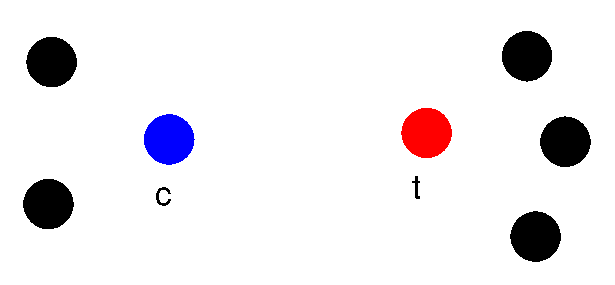
\includegraphics[width=5cm]{./Drawn/RcdlNnRnnEg}
\end{figure}
For $k=3$:
\begin{itemize}
	\item $ t \in NNs(c) $
	\item $ c \in rNNs(t) $
\end{itemize}
\end{samepage}

\subsection{Classifies / Misclassifies}
\subsubsection{Case Contribution\label{sec:contributes}}
A case $c_{2}$ \emph{contributes} to another case $c_{1}$'s classification if $c_{2}$ is retrieved as a nearest neighbour of $c_{1}$ and $c_{2}$ aids `positively' to $c_{1}$'s classification (i.e. is the same label as $c_{1}$ if $c_{1}$ is correctly classified, or is a different label to $c_{1}$ if  $c_{1}$ is incorrectly classified).
\subsubsection{Classifies}
\begin{quote}
$ Classifies(t, c) $ means that case $c$ contributes to the correct classification of target case $t$. This means that target case $t$ is successfully classified and case $c$ is returned as a nearest neighbour of case $t$ and has the same classification as case $t$ \citep{Delany2009}.
\end{quote}

Therefore, for $ Classifies(t, c) $:
\begin{enumerate}
	\item $t$ must be correctly classified by the case-base.
	\item $c$ must be returned as a neighbour of $t$ in that correct classification.
	\item $c$ must be of the same label as $t$'s actual label\footnote{By ``actual label'', we mean the label that the instance actually has, irrespective of how the case-base classifies it.}.
\end{enumerate}

\subsubsection{Misclassifies}

\begin{quote}
$ Misclassifies(t, c ) $ means that case $c$ contributes in some way to the incorrect classification of target case $t$. In effect this means that when target case $t$ is misclassified by the case-base, case $c$ is returned as a neighbour of $t$ but has a different classification to case $t$ \citep{Delany2009}.
\end{quote}


Therefore, for $ Misclassifies(t, c) $:
\begin{enumerate}
	\item $t$ must be incorrectly classified by the case-base.
	\item $c$ must be returned as a neighbour of $t$ in that classification.
	\item $c$ must be of a different label than $t$'s actual label.
\end{enumerate}

\subsubsection{Example}

In the example presented in Figure \ref{fig:equaldistancemisclassifieseg}, the case $x$ is incorrectly classified as a circle by the case-base (with k=6). Here, the 3 circles (c2, c3 and c4) and the 1 square (c1) contribute to the incorrect classification, and thus:
\begin{itemize}
	\item $Misclassifies(x,c)~\forall c\in\{c1,c2,c3,c4\}$
\end{itemize}

\begin{figure}[h!] \centering
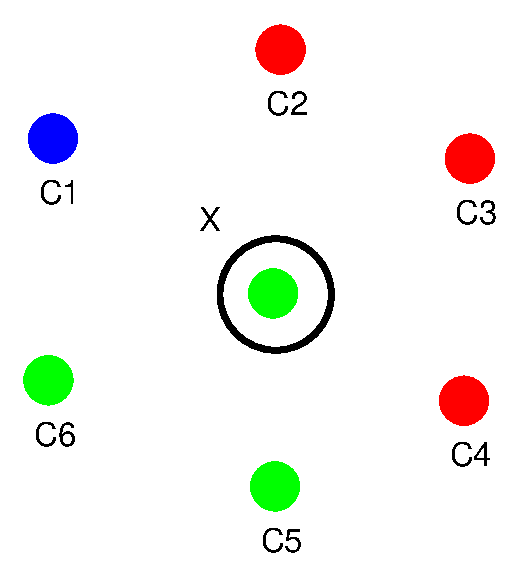
\includegraphics[width=120pt]{./Drawn/EqualDistanceMisclassifiesEg}
\caption{Example of case-base incorrectly classifying a case. x is classified as a Circle by the case-base, whereas its actual label is a Triangle.}
\label{fig:equaldistancemisclassifieseg}
\end{figure}

\subsection{RCDL Definitions}
Reachability and coverage relate to cases being correctly classified by the case-base, whereas dissimilarity and liability relate to cases being incorrectly classified by the case-base.

Reachability and dissimilarity are concerned with the NNs of a case, whereas coverage and liability are concerned with the rNNs of a case.

\subsubsection{Reachability Set}
\[ ReachabilitySet(c \in C) = \left\lbrace t \in C : Classifies(c, t) \right\rbrace \] 
If $c$ is correctly classified by the case-base, these are all the cases in $ NNs(c) $ that have the same label as $c$. Otherwise, this set is empty (and the Dissimilarity set is instead populated).

\subsubsection{Coverage Set}
\[ CoverageSet(c \in C) = \left\lbrace t \in C : Classifies(t, c) \right\rbrace \]
These are all the cases $ t \in rNNs(c) $ such that $t$ is correctly classified by the case-base and the label of $t$ is the same as the label of $c$.

\subsubsection{Dissimilarity Set}
\[ DissimilaritySet(c \in C) = \left\lbrace t \in C : Misclassifies(c, t) \right\rbrace \]  
If $c$ is incorrectly classified by the case-base, these are all the cases in $ NNs(c) $ that have a different label than the actual label of $c$. Otherwise, this set is empty (and the reachability set is instead populated).

\subsubsection{Liability Set}
\[ LiabilitySet(c \in C) = \left\lbrace t \in C : Misclassifies(t, c) \right\rbrace \]  
These are all the cases $ t \in rNNs(c) $ such that $t$ is incorrectly classified by the case-base, and the label of $c$ is different from the label of $t$.

\section{Delaney's Analysis}

\subsection{Case Classifications}
Through the definitions of the RCDL sets - Delaney notes the following \citep{Delany2009}\footnote{The following profile analysis is taken verbatim from the cited paper. They gives a good break-down of the possibilities, and are simply useful to keep in mind when considering the rest of the RCDL approach - hence their inclusion.}:

\begin{enumerate}
	\item Firstly, it is possible to indicate whether the case is correctly or incorrectly classified by the case-base. This is identified by the case having either a non-empty reachability set (R) or a non-empty dissimilarity set (D).
	\item Secondly, we can consider whether the case is useful, by the existence of a non-empty coverage set (C), and
	\item Finally whether the case is harmful and causes damage, by the existence of a non-empty liability set (L).
\end{enumerate}

Through enumeration of the possible RCDL Combinations, 8 possible profiles exist for a case, using the occurrence of a non-empty set as the \emph{flag} on which to enumerate \citep{Delany2009}:

\begin{enumerate}
	\item \emph{R}: A case which is correctly classified but is not used for classifying any other case in the case-base.
	\item \emph{D}: A case which is misclassified but is not used for classifying any other case in the case-base.
	\item \emph{RC}: A case which is correctly classified and is useful in that it has contributed to the correct classification of other cases in the case-base. This profile and the R profile are generally the majority case profile types.
	\item \emph{RL}: A case which is correctly classified but is harmful in the case-base causing damage by contributing to other cases being misclassified.
	\item \emph{DC}: A case which is misclassified but is useful in the case-base. 
	\item \emph{DL}: A case which is misclassified and is harmful in the case-base.
	\item \emph{RCL}: A case which is correctly classified and is both useful and harmful in the case-base.
	\item \emph{DCL}: A case which is misclassified and is both useful and harmful in the case-base.
\end{enumerate}


\subsection{Experimental Conclusions}
In her experiments, Delaney investigates the effect of removing cases with different RCDL profiles on case-base competence. She also compares her strategies with other noise-removal strategies, and frames them in RCDL terms.

While the specific results vary between datasets, Delaney notes that there was a consistent improvement with the removal of just DL \& DCL cases from the datasets. 

The reader is recommended to consult \citet{Delany2009} for the thorough analysis. For the purpose of our work, the specific results are not of great importance, since we wish to try using the RCDL profiles for in a pool-based active learning scenario.

\section{Continuing From Delaney's Work}
The simplicity of the boolean set-non-emptiness characteristic of the case profiles Delaney defines has its merits. It is relatively easy to understand and reason about. 

It does, however, throw away a lot of potentially useful information by not trying to do any reasoning about the contents of the sets.

In our work, we expand on the RCDL approach by using it in a non-boolean way for active learning selection strategies.

\section{RCDL Consequences}

\subsection{Either-or Nature of reachability and dissimilarity sets}
If a case has a non-empty reachability set then it has been classified correctly by the case-base and, as such, will have an empty dissimilarity set and vice versa.

Intuitively, these sets simply represent the set of cases that contribute to a case's classification (with the notion of \emph{contributes} as outlined in section \ref{sec:contributes}). 

If the case is correctly classified, this set is referred to as the reachability set, whereas if incorrectly classified, it is referred to as the dissimilarity set.

\subsection{Reachability-Coverage / Liability-Dissimilarity Duality\label{sec:duality}}
Simply put, if case $c$ occurs in case $t$'s reachability set, case $t$ occurs in $c$'s coverage set. Similarly with liability and dissimilarity.
The reasoning is as follows:
\begin{itemize}
	\item Take a single case pair, $c1$ and $c2$ such that $Classifies(c1, c2)$.
	\begin{itemize}
		\item $c2$ contributes to the correct classification of $c1$.
	\end{itemize}
	\item From $c2$'s perspective, $c1$ is in its coverage set.
	\begin{itemize}
		\item From the formula above, from $c2$'s perspective, $c=c2$, and $t=c1$, and it is the case that $Classifies(t, c)$.
	\end{itemize}
	\item From $c1$'s perspective, $c2$ is in its reachability set.
	\begin{itemize}
		\item From the formula above, from $c1$'s perspective, $c=c1$ and $t=c2$, and it is the case that $Classifies(t, c)$.
	\end{itemize}
\end{itemize}

Similar reasoning can be applied to the liability and dissimilarity sets.

This point is easier to understand just by intuition around the plain-English definitions of the RCDL profiles above.

\subsection{Reachability is to Dissimilarity as Coverage is to Liability}
This is obvious from looking at the formulas, but is worth pointing out for future notes.

\subsection{Reachability/Dissimilarity concerned with Nearest Neighbours, Coverage/Liability with Reverse Nearest Neighbours \label{sec:RdWithNnClWithRnn}}
This can simply be derived from the definitions above, but of primary note is that:
\begin{itemize}
	\item The reachability and dissimilarity sets of a case can be inferred by just looking at that case's nearest neighbours.
	\item The coverage and liability sets of a case can be inferred by just looking at that case's reverse nearest neighbours\footnote{This is assuming the case-base's classification of each of the reverse nearest neighbours is known. In our later work, it will be, as it will be cached from previous classification.}.
\end{itemize}

\subsection{Max Size of Reachability and Dissimilarity sets bounded to K}
Given that the reachability and dissimilarity sets of a case are always subsets of that case's NNs, the maximum size is K - the size of the NNs set\footnote{This is assuming that a \emph{strict} KNN is used, where at max k neighbours are used even when ties exist.}.

\section{An Incremental Strategy to RCDL\label{sec:incrstrategy}}
\subsection{Justification} 
In Delaney's work, it was sufficient to calculate the case-base RCDL profiles in a brute-force manner, since it was the most efficient way in her case-base maintenance investigation on existing case-bases. For selection strategies this would not hold, since the profiles would need to be inferred many times for a changing case-base.

It would also be useful to be able to determine what RCDL changes would occur in the RCDL profiles if a new case was added with a given label. If this were to be done for each unlabelled case when selecting a case to add to the case-base, it would be very expensive to re-build the entire set of RCDL profiles for the case-base each time.

Thus, we decided to create an incremental strategy in which the changes can also be inferred in linear time before actually \emph{adding} a case to the case-base.

\subsection{Desired Algorithm Structure}
\subsubsection{Inputs}
\begin{itemize}
	\item A case-base 
	\item k - the size of the neighbourhood
	\item RCDL, NN, and rNN profiles for each of the cases
\end{itemize}

\begin{samepage}
For the remainder of this algorithm description, the term `profile' is used to denote the RCDL profile with the NNs and rNNs:
\nopagebreak[4]
\begin{code}[numbers=none,frame=none]
CaseProfile:  
  Reachability Set:  \{...\}
  Coverage Set:      \{...\}
  Dissimilarity Set: \{...\}
  Liability Set:     \{...\}
  NNs:               \{...\}
  rNNs:              \{...\}
\end{code}
\end{samepage}
\subsubsection{Operations\label{sec:incralgstructops}}
\paragraph{$Suppose(unlabelled\_instance, label)$:}
This operation should determine what changes would occur to the profiles of the cases in the case-base if a given unlabelled instance was added to the case-base with a given label\footnote{The label for the unlabelled instance will not be known prior to consulting the oracle, so we only want to perform ``What-if'' analysis - i.e. ``What would happen happen if I added this case to the case-base, and it turned out to be this label''.}.

A Change to a given case may be denoted as the pair (Added, Removed), where Added and Removed in turn are simply partial profiles:
\begin{code}[numbers=none,frame=none]
Change:
  Added:
    Reachability Set:  \{...\}
    Coverage Set:      \{...\}
    Dissimilarity Set: \{...\}
    Liability Set:     \{...\}
    NNs:               \{...\}
    rNNs:              \{...\}
  Removed:
    Reachability Set:  \{...\}
    Coverage Set:      \{...\}
    Dissimilarity Set: \{...\}
    Liability Set:     \{...\}
    NNs:               \{...\}
    rNNs:              \{...\}
\end{code}

The output for this algorithm will be a set of (Case, Change) pairs. For algorithmic ease, this also includes the input unlabelled case, since technically, adding it will cause cases to be added to its reachability set, etc. But understandably, for the input case's Change, the Removed data will always be empty.

\paragraph{$Add(labelled\_case)$:}
This operation simply adds a given case to the case-base, updating the case-base's profiles as appropriate. Operationally, this involves supposing that the case was added with its label using the previous suppose operation, and updating the case-base's profiles as per the returned set of (Case, Change) pairs.


\subsection{Algorithm Outline}
The rough approach taken is to first determine the changes which occur to NNs and rNNs. From these, along with knowledge of the existing RCDL profiles, the changes to reachability, coverage, dissimilarity and liability are inferred\footnote{For clarity, the outline refers to updating the actual case-base profiles collection, whereas really it's a Change object for each one that it modifies, and finally returns. While, at this stage, this is simply an implementation detail, it will become important when we start using the suppose operation (Section \ref{sec:actofsupposing}).}.

\subsection{Figuring out NN / rNN changes}
\subsubsection{Overview}
When a case is added to the case-base, figuring out the nearest neighbour and reverse nearest neighbours changes essentially involves two steps:
\begin{enumerate}
	\item Determine the new case's nearest neighbours, and for each NN, add the new case to NN's reverse nearest neighbours set.
	\item Determine the existing cases of the case-base that have the new case as a nearest neighbour, and deal with the change appropriately.
\end{enumerate}

The second step is trickier than the first, since the new case may have displaced an existing case from the NNs set, therefore this needs to be taken into account when maintaining consistency of NNs to rNNs in all cases concerned.

\subsubsection{Algorithm\label{sec:nnchangesalg}}
\begin{code}
// Sort out the new case's nearest neighbours
Determine new case's NNs
For each NN of the new case's NNs:
  add the new case to the NN's rNNs

// Sort out the new case's reverse nearest neighbours.
For each existing case that has the new case as an NN:
  Add the existing case to the new case's rNNs
  Add the new case to the existing case's NNs
  If the new case shunted an NN of the existing case:
    Remove shunted case from the existing case's NNs
    Remove existing case from the shunted case's rNNs
\end{code}

\subsubsection{Algorithm Notes}
\paragraph{Determining if an existing case has the new case as an NN within k}
Unfortunately, each case in the case-base needs to be examined to determine if it has the new case as an NN. But because we have the NNs stored for each case in the case-base, the examination of each case can be a relatively quick operation, versus the alternative of having to, for each case, go through the entire case-base to find its NNs if they weren't stored.

The maximum NN distance in the cached NN list need only be compared to the distance of the new case, with consideration for tie breaking as in the KNN classifier if they're equal.

\paragraph{Duality of NN/rNN changes (both added and removed)}
If a case has a nearest neighbour added, then that nearest neighbour will get a reversed nearest neighbour added. Thus, for any NN add, there is a corresponding rNN add. Similarly for remove.

This allows us just to iterate through the NN changes, and infer the presence of the corresponding rNN change as a result.

\paragraph{NN Shunting}
We define a case $A$ as \emph{shunting} another case $N$ from the NNs set of $B$ if $N$ is removed as a nearest neighbour of $B$, and $A$ added.

An example can be found by looking at Figure \ref{fig:flipprecedence}. Here, for $k=3$S, $Cn$ \emph{shunts} $C1$ from $Cp$'s NNs set.

\subsection{The Incremental RCDL Profile Building Algorithm}

\subsubsection{Overview}
The algorithm uses the NN/rNN changes determined using the previous algorithm (Section \ref{sec:nnchangesalg}), and goes through each NN change\footnote{Because of NN/rNN duality - changes to rNNs, and sets relating to rNNs (coverage and liability), can be inferred.}, handling individually. The core of the algorithm proceeds in roughly two parts:
\begin{enumerate}
	\item Deal with the NN removals first
	\item Deal with the NN additions, taking into account scrubbing and the effect of classification changes.
\end{enumerate}

The primary issue that requires careful consideration is when the addition of the new case causes the classification of an existing case in the case-base to change - since the RCDL profiles relate heavily to whether a case has been correctly classified or not.

\newpage
\subsubsection{Algorithm} \nopagebreak[4]
\begin{code}
Compute the NN/rNN changes using the suppose_nn algorithm.
foreach case in the NN/rNN changes:
  // Deal with NN removals, if present
  foreach removed_case in case's NN removals:
    if the removed_case was in case's reachability set:
      Remove removed_case from case's reachability set
      Remove case from removed_case's coverage set.
    else if removed_case was in case's dissimilarity set:
      Remove removed_case from case's dissimilarity set
      Remove case from removed_case's liability set.

  // Deal with NN additions, if present  
  Calculate case's new classification
  if the case's correct-classification-status changed:
    // Need to scrub appropriate RCDL sets
    for each r in the case's old `contributors' list:
      if the case's old classification was correct:
        Remove r from case's reachability set
        Remove case from r's coverage set
      else:
        Remove r from case's dissimilarity set
        Remove case from r's liability set
        
  for each c in the case's new `contributors' list:
    if the case's new classification is correct:
      Add c to case's reachability set
      Add case to c's coverage set
    else:
      Add c to case's dissimilarity set
      Add case to c's liability set
\end{code}

\subsubsection{Algorithm Notes}
\paragraph{Ability to just look at NN changes}
Due to the NN/rNN Duality property described above with regards NN changes, any NN add is guaranteed to have an rNN add, and similarly with remove. This allows us to consider only NN changes, and while dealing with an NN change, deal with the corresponding rNN change.

\begin{samepage}
\paragraph{Permutations of NN changes}
Because of the previous note, we only really need to deal with the added and removed nearest neighbours. The following are the permutations of NN changes, following `supposing' the addition of a single case:

\vspace{10pt}

\begin{tabular}{ | c | c | p{280pt} |} \hline
	NN Added & NN Removed & Notes \\ \hline
	1 & 1 & Will be the only type when $\left|CaseBase\right|> k$. \\ \hline
	1 & 0 & Happens only at the start, when $\left|CaseBase\right|\leq k$. \\ \hline
	0 & 1 & Can never actually happen - there would have to be another Case to replace the removed one since we're only dealing with adding a case to the case-base. \\ \hline
	0 & 0 & Uninteresting - its rNNs will be covered elsewhere with the corresponding NN changes of another case. \\ \hline
\end{tabular}

\end{samepage}

\paragraph{An NN Removal Guarantees an NN Add}
This can be seen in the truth table above. Because we're only dealing with a new case being added, the effect of the new case can never cause an NN removal without causing a corresponding NN add of the new case. Because of having a shorter distance to the target case than the furthest-distance NN, the new case will have \emph{shunted} that NN - causing an NN removal.

This allows us to not worry about, at the stage of dealing with NN removals, if the removal caused the label to change, because we'll be dealing with that scenario anyway in the corresponding add.

\paragraph{An NN removal might affect R/D of case in question, C/L of other}

For the following example,
\begin{itemize}
	\item $k=3$, 
	\item $x$ is the case in question whose NNs  we'll talk about
	\item $y$ is the new case added to the case-base
	\item $c1$, $c2$, $c3$ are the NNs of $x$ prior to $y$ being added
	\item $c1$ is the \emph{shunted} case which is removed from NNs(x) after $y$ is added.
\end{itemize}

\begin{figure}[h!] \centering
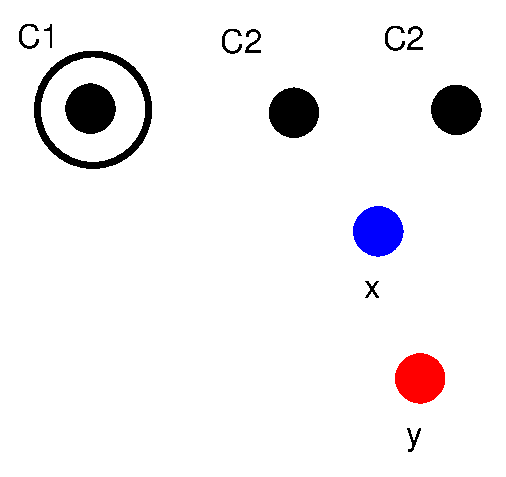
\includegraphics[width=5cm]{./Drawn/NnMightAffectEg}
\end{figure}

$c1$ was an NN of $x$, and $x$ was an rNN of $c1$. As described previously in \ref{sec:RdWithNnClWithRnn}, a case's NNs can affect its reachability / dissimilarity sets, whereas a case's rNNs can affect its coverage / liability sets. So the removal of $c1$ as an NN of $x$ (and the corresponding removal of $x$ as an rNN of $c1$) might affect $c1$'s reachability / dissimilarity set, and $x$'s coverage / liability set, because when $c1$ is removed as an NN, it can't contribute either positively or negatively any more to $x$'s classification.\footnote{Note that it is not guaranteed that $c1$ was in $x$'s reachability / dissimilarity set, or that, equivalently, $x$ was in $c1$'s coverage / liability set. The sets will only be affected if $c1$ was a \emph{contributor} of $x$'s classification by the case-base. Hence the usage of ``might affect''.}

All this leads to a simple way to dealing with an NN removal \footnote{The corresponding NN addition will be dealt with separately}:
\begin{itemize}
	\item If $c1$ was in $x$'s coverage / liability set, it should be removed.
	\item If $x$ was in $c1$'s reachability / dissimilarity set, it should be removed.
\end{itemize}

\paragraph{Calculating a case's new classification}
This can be done semi-intelligently since a case's old NNs are known. Instead of doing KNN classification with the entire case-base, we only need to look at a case's new NNs (which can be inferred from its old NNs and the NN changes) to determine the new classification.

\paragraph{Correct-classification-status}
We will furthermore commonly talk about a case's correct-classification-status as opposed to its classification alone. It simply means whether a case has been correctly classified by the case-base or not. 

\paragraph{A case's correct-classification-status determining reachability/dissimilarity}
If a case is correctly classified by the case-base, its reachability set will be populated. If it is incorrectly classified, its dissimilarity set will be populated.
 
\paragraph{Effect of a correct-classification-status changing}
Firstly, we need only worry about if the correct-classification-status of a case changes with the addition of a new case, as opposed to if the classification alone changes.

For example, if a case's actual label was `triangle', it was previously classified `square', and with the addition of the new case, it's classified `circle', it has still been incorrectly classified both before and after the addition of the new case, therefore we do not need to worry about scrubbing.

If however the correct-classification-status of a case $c$ does change, we need to perform \emph{scrubbing} on some of the RCDL sets.

If it went from correctly classified to incorrectly classified:
\begin{itemize}
	\item $c$'s reachability set needs to be scrubbed (all items removed).
	\item For each \emph{scrubbed} case from the reachability set, the scrubbed case needs to have $c$ removed from its coverage set.
	\item $c$'s dissimilarity set needs to be populated with the elements in its new NNs that have a different label to its actual label.
	\item For each thing put in the dissimilarity set, their liability sets need to have $c$ added.
\end{itemize}

Similarly, if it went from incorrectly classified to correctly classified:
\begin{itemize}
	\item $c$'s dissimilarity set needs to be scrubbed (all items removed).
	\item For each \emph{scrubbed} case from the dissimilarity set, the scrubbed case needs to have $c$ removed from its liability set.
	\item $c$'s reachability set needs to be populated with the elements in its new NNs that have the same label as its actual label.
	\item For each thing put in the reachability set, their coverage sets need to have $c$ added.
\end{itemize}

\paragraph{Not allowing supposing of an already present case}
The algorithm presented does not allow for an already present case in the case-base to be \emph{supposed} (e.g. if x is in the case-base with label `square', what would happen if x was actually `circle').

\paragraph{Not allowing for supposing the removal of a case}
The algorithm presented does not allow for supposing the removal of a case from the case-base (e.g. what would happen if I removed x from the case-base?), though it could be updated to support this scenario.

\subsection{Testing and Validation}
Testing was performed in Unit-Test style to ensure the RCDL profiles achieved using the incremental strategy presented correlated exactly with a simple brute-force strategy. This was done on each of the datasets used.

\vspace{10pt}

\begin{samepage}
\subsubsection{Brute Force Algorithm}
\begin{code}
// Compute NNs and rNNs
foreach case in case_base:
  case_rcdl = case's RCDL Profile
  case_nns = the k-nearest neighbours of case
  Add case_nns into case_rcdl.nearest_neighbours
  foreach nn in case_nns:
    nn_rcdl = nn's RCDL Profile
    case_to_profile_dict[nn].reverse_nearest_neighbours.add(case)

// From NNs & rNNs, compute the remainder of the RCDL Profiles
foreach case in case_base:
  case_rcdl = case's RCDL Profile
  actual_label = oracle(case)
  classified_label = Classify using case_rcdl.nearest_neighbours
  case_rcdl.classification = classified_label
  
  if actual_label == classified_label:
    helping_cases = \{nn for nn in case_rcdl.nearest_neighbours 
                     if oracle(nn) == actual_label\}
    Add helping_cases to case_rcdl.reachability_set
    foreach hc in helping_cases:
      hc_rcdl = hc's RCDL Profile
      Add case to hc_rcdl.coverage_set
  else:
    hurting_cases = \{nn for nn in case_rcdl.nearest_neighbours 
                     if oracle(nn) != case_actual_label\}
    Add hurting_cases to case_rcdl.dissimilarity_set
    foreach hc in hurting_cases:
      hc_rcdl = hc's RCDL Profile
      Add case to hc_rcdl.liability_set
\end{code}
\end{samepage}

\medspace
\vspace{10pt}

\pagebreak
\subsubsection{The Test}
\nopagebreak[4]
\begin{code}
Shuffle the dataset
incremental_builder = A new instance of the Incremental RCDL Builder
case_base = \{\}

foreach case in dataset:
  Add case to case_base
  
  // Use the incremental builder to get the rcdl profiles
  profile_builder.put(case)
  incr_profiles = profile_builder.case_profiles
  
  // Use Brute Force to get the rcdl profiles
  bf_profiles = Build the profiles brute force from the case_base
  
  // Make sure that they're the same size so I don't 'miss' any
  assert that |br_profiles| == |incr_profiles|
  
  // Iterate through each profile, and make sure its 
  // brute force equivalent is the same
  for (pb_case, pb_case_profile) in incr_profiles:
      bf_case_profile = Get pb_case's case profile from bf_profiles
      assert that pb_case_profile == bf_case_profile
\end{code}

\subsubsection{Timings}
\begin{figure}[h!] 
\centering
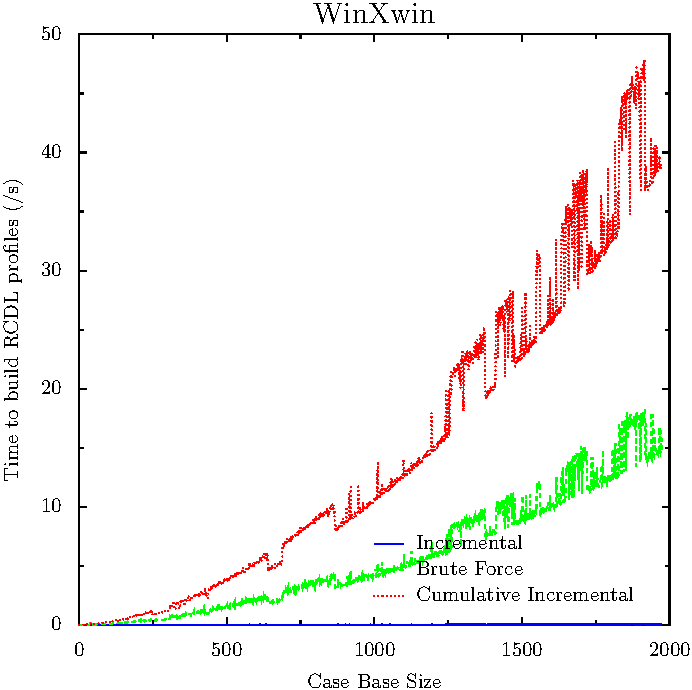
\includegraphics[width=300pt]{./ExperimentResults/WinXwin_timings_all}
\caption{Plot of timings information for brute force algorithm, incremental algorithm, and the cumulative time of the incremental algorithm on dataset `WinXwin'}
\label{fig:winxwintimingsall}
\end{figure}

\begin{figure}[h!] 
\centering
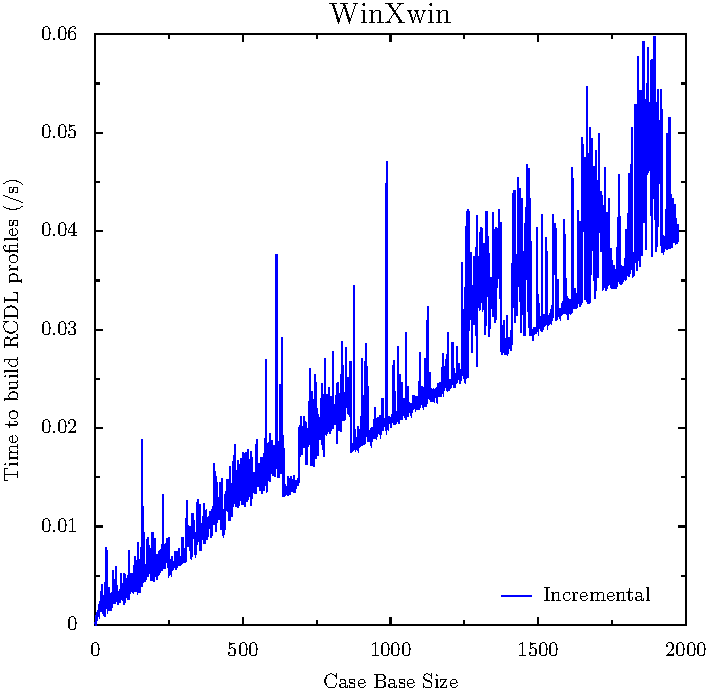
\includegraphics[width=300pt]{./ExperimentResults/WinXwin_timings_incr_only}
\caption{Plot of timings information for incremental algorithm on dataset `WinXwin'}
\label{fig:winxwintimingsincronly}
\end{figure}

\begin{samepage}
As can be seen in Figure \ref{fig:winxwintimingsall}, using the incremental algorithm to add a single case to the case-base is much faster than re-building the entire profile collection from scratch. There is however an overhead to using the incremental strategy, as can be seen by the cumulative times. For general application, it is thus better to use a brute force style if the profiles need only be computed once ever, but if the case-base is being continually modified, and the profiles needed, the incremental strategy has its obvious merits.

Figure \ref{fig:winxwintimingsincronly} shows a plot of just the incremental timings, since it is difficult to make out in Figure \ref{fig:winxwintimingsall}.
\end{samepage}

%\subsubsection{Complexity Analysis}
%TODO Write the Complexity Analysis Section.

\chapter{Competence Based Selection Strategies\label{cha:compbasedselstrategies}}
\section{Types of RCDL Changes from adding a Single Case to the Case-Base}
\subsection{NNs of the New Case}
\begin{figure}[h!] 
\centering
	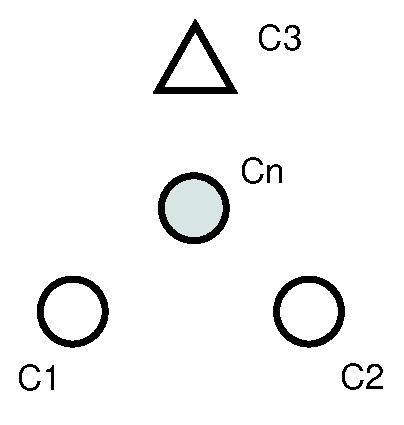
\includegraphics[width=100pt]{./Drawn/NNsCorrectlyClassify}
\caption{Nearest neighbours causing the correct classification of a case as a Circle.}
\label{fig:NNsCorrect}
\end{figure}

In the example presented in Figure \ref{fig:NNsCorrect}, the NNs of the added case Cn are \{C1, C2, C3\}. Cn is correctly classified by the case-base as a circle, thus we are dealing with the reachability and coverage sets.
\begin{itemize}
	\item Cn will have a reachability set consisting of the cases which contribute to its correct classification - \{C1, C2\}.
	\item Similarly, because C1 and C2 both contribute to the correct classification of Cn, they will have Cn added to both their coverage sets.
\end{itemize}

If Cn had been incorrectly classified - it would instead have been the dissimilarity and liability sets affected - e.g.

\begin{figure}[h!]
  \centering
	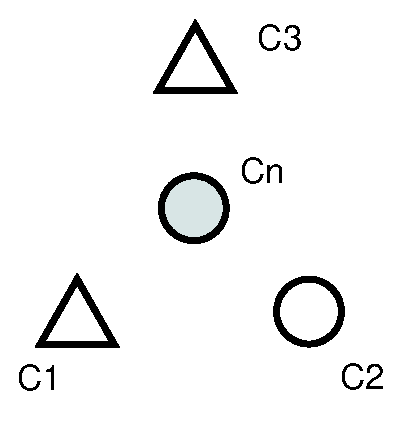
\includegraphics[width=100pt]{./Drawn/NNsIncorrectlyClassify}
\caption{Nearest neighbours causing the incorrect classification of a case as a Triangle.}
\label{fig:nnsincorrectlyclassify}
\end{figure}

In the example presented in Figure \ref{fig:nnsincorrectlyclassify}, C3 and C1 contribute to the incorrect classification of Cn, so
\begin{itemize}
	\item Cn will have a dissimilarity set consisting of \{C3, C1\}.
	\item Similarly, Cn will be added to C3 and C1's liability sets.
\end{itemize}

\subsection{rNNs of the New Case}
The rNN related changes are somewhat trickier, since they are not bounded to k, and have the potential to have knock-on effects to other cases not directly related to the new case.
The running example throughout will be as follows:

\begin{figure}[h!] 
\centering
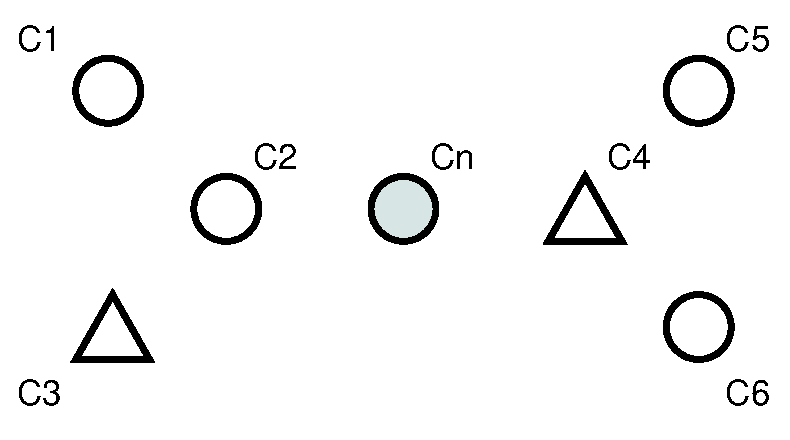
\includegraphics[width=200pt]{./Drawn/rNNExample}
\end{figure}

k = 3, and distance weighted voting is used. C2 and C4 will be the primary cases of interest, with Cn the new case added (or supposed).

Before Cn's addition, C2 was incorrectly classified by the case-base as a triangle, with C3 and C4 contributing to it, and C4 incorrectly classified as a circle, with C2, C5 and C6 contributing to it.

After Cn's addition, C2 is correctly classified by the case-base, with C1 and Cn contributing to it and C4 is still incorrectly classified by the case-base, but now with Cn, C5 and C6 contributing to it.

\subsubsection{Direct\label{sec:direct}}
When a new case is added to the case-base, it may contribute in some fashion to the classification of some of its rNNs.

In the example, C2 is correctly classified by the case-base as a circle, and Cn, the new case added, contributes to the correct classification. As a result,
\begin{itemize}
	\item Cn's coverage set will have C2 added to it, 
	\item C2's reachability set will have Cn added to it
\end{itemize}

C4, on the other hand, is incorrectly classified by the case-base, and the new case Cn is contributing to it.
\begin{itemize}
	\item Cn's liability set will have C4 added to it,
	\item C4's Dissimilarity set will have Cn added to it.
\end{itemize}

\subsubsection{Case NN Shunting}
When a new case is added to the case-base, it is possible that it will become one of an existing case's nearest neighbours, and `shunt' some other case for the position, i.e. the `shunted' case was an NN of some case, but after the new case is added, it is not. Here, we talk about actions relative to the case for which its NNs changed as a result of the new case being added.

In the example, C2, C5 and C6 were the contributing neighbours to C4's incorrect classification as a circle. When Cn was added, it was closer to C4 than C2, and so C2 was removed as an NN, and Cn added. Cn too contributes to C2's incorrect classification.  As a result of the NN changes: 
\begin{itemize}
	\item C2 is removed from C4's dissimilarity set  
	\item C4 is removed from C2's liability set
	\item Cn is added to C4's dissimilarity set (covered under Direct as in Section \ref{sec:direct})
	\item C4 is added to Cn's liability set (covered under Direct as in Section \ref{sec:direct})
\end{itemize}


\begin{tabular}{|x{40pt}|x{40pt}|x{280pt}|}
\hline 
\raggedright{{\small Case Correctly Classified}} & \raggedright{{\small Shunted Contrib'd}} & {\small Action}\tabularnewline 
\hline 
1 & 1 &
\begin{itemize}
	\item \textit{Shunted} removed from \textit{case}'s reachability set
	\item \textit{Case} removed from \textit{Shunted}'s coverage set
\end{itemize} \tabularnewline
\hline 
0 & 1 & 
\begin{itemize}
	\item \textit{Shunted} removed from \textit{case}'s dissimilarity
	\item \textit{Case} removed from \textit{Shunted}'s liability
\end{itemize} \tabularnewline
\hline 
0 & 0/1 & Uninteresting. A case was shunted, but it didn't contribute previously, so it will be unaffected by the shunting. \tabularnewline
\hline 
\end{tabular}

\subsubsection{Correct-Classification-Status Flip}
The new case's rNNs might have changed their correct-classification-status due to the addition of the new case. This may result in other cases not directly related to the new case, but instead related to the rNN, to be affected.

In the example, C2 was incorrectly classified as a triangle before the addition of Cn, with C3 and C4 the contributors to this classification. After Cn is added, its classification changes to the correct classification - a circle. We say that its correct-classification-status has changed. As a result, C1 now contributes to the classification (in addition to the new case Cn), and C3 does not. C4 was shunted from its position and is covered instead under Case NN Shunting.

Changes as a result in particular of the correct-classification-status flip:
\begin{itemize}
	\item C3 is removed from C2's dissimilarity set
	\item C2 is removed from C3's liability set
	\item C1 is added to C2's reachability set
	\item C2 is added to C1's coverage set
\end{itemize}

In addition, the effect of ``NN Shunting'' and ``Direct'' come into play with respect to C2:
\begin{itemize}
	\item C4 is removed from C2's dissimilarity set (NN Shunting)
	\item C2 is removed from C4's liability set (NN Shunting)
	\item Cn is added to C2's reachability set (Direct)
	\item C2 is added to Cn's coverage set (Direct)
\end{itemize}

\begin{tabular}{|x{55pt}|x{355pt}|}
\hline 
Change & Action \tabularnewline 
\hline 
Correct to Incorrect & 
\begin{itemize}
	\item The case's reachability set needs all items removed from it.
	\item Each item removed needs to have the case removed from its coverage set.
	\item The case's dissimilarity set needs all NNs of a different label added to it.
	\item Each item added needs to have the case added to its liability set.
\end{itemize} \tabularnewline 
\hline 
Incorrect to Correct & 
\begin{itemize}
	\item The case's dissimilarity set needs all items removed from it.
	\item Each item removed needs to have the case removed from its liability set
	\item The case's reachability set needs all NNs of a different label added to it.
	\item Each item added needs to have the case added to its coverage set.
\end{itemize} \tabularnewline 
\hline 
\end{tabular}	

\subsection{RCDL Change Possibility Matrix from a Case Addition\label{sec:rcdlchangematrix}}
\begin{tabular}{|c|c|c|c|c|c|}
\cline{4-6} 
\multicolumn{1}{c}{} & \multicolumn{1}{c}{} &  & \multicolumn{3}{c|}{Existing Cases}\tabularnewline
\cline{3-6} 
\multicolumn{1}{c}{} &  & New Case & Direct & Shunt & Flip\tabularnewline
\hline
\multirow{2}{*}{Any RCDL Set} & Add & X & X &  & X\tabularnewline
\cline{2-6} 
 & Remove &  &  & X & X\tabularnewline
\hline 
\end{tabular}

\vspace{12pt}

The above table summarises in brief the findings of the possible types of changes that can happen from adding a new case the case-base. For example:
\begin{itemize}
	\item The mark corresponding to ``New Case'', ``Add'' means that, as a result of the addition of the new case, any of the new case's RCDL sets might have elements added to them.
	\item The mark corresponding to ``Existing Cases Shunt'', ``Remove'' means that, as a result of the addition of the new case, shunt type changes can involve removing cases from the RCDL sets of the existing cases.
	\item The absence of the mark corresponding to ``Existing Cases Shunt'', ``Add'' means that RCDL sets of existing cases will not be added to as a result of Shunt type changes as defined previously.
\end{itemize}

The table may simply be used as a reference when considering the formulae presented later when describing competence selection strategies.

\section{Selection Strategy Pre-Notes}
\subsection{The Act of Supposing\label{sec:actofsupposing}}
When an unlabelled case is evaluated for inclusion in the case-base, the actual label for the case is unknown. It could have any of the possible labels. As a result, when considering a case for inclusion, it is desirable to evaluate its benefit for all possible labels, possibly considering the likelihood of the label given what we already know through the case-base.

\subsection{Measure Deviation between the Possible labels}
For some strategies, the deviation between the changes for the different possible labels is also of interest.

\subsection{Categorizing Suppose Changes}
It should first be noted that, due to the occurrence of Shunt and Flip type changes, a single case change (as described in Section \ref{sec:incralgstructops}) can concurrently contain multiple RCDL change types.

It would be useful for when developing new selection strategies to be able to determine whether a particular change were a `Direct', `Flip' or `Shunt'.

\subsubsection{Suppose Change Set SFD Categorization Algorithm}
\begin{code}
Algorithm CategorizeChanges(change_pairs, new_case):
  let (direct_cps, shunt_cps, flip_cps) = (\{ \}, \{ \}, \{ \})
  for (existing_case, change) in change_pairs:
    if existing_case == new_case:
      // All changes regarding the new case are regarded as Direct, 
      // no extra work needed
      direct_cps[existing_case] = change)
      continue

    // Want to iterate over all changes (both added and removed) 
    // of reachability and dissimilarity, and categorize each 
    // case change individually
    for (rcdl_set, op) in cross product of 
                          \{`reachability', `dissimilarity`\} 
                      and \{`Added', `Removed'\}:
      for other_case in `op' of `rcdl_set' of change:
        if other_case == new_case:
          let change_type = `direct'
        else if correct-classification-status did change 
             and (other_case contributed to existing_case's
                      previous classification):
          let change_type = `flip'
        else:
          let change_type = `shunt'
          
        Add this change to existing_case pair in change_type's CPs set 
            (i.e. shunt_cps, flip_cps or direct_cps)
    
  // All reachability and dissimilarity sets have been dealt with,now we
  // need to use the reachability and dissimilarity sets of each to infer
  // and make the changes for coverage and liability changes.
  for cps in (direct_cps, shunt_cps, flip_cps):
    PlaceDuals(cps)
\end{code}

\subsubsection{Flips taken to `overpower' Shunts}
If a correct-classification-status flip occurs for a case, and the shunted case would have been removed by the flip anyway, even if it were not shunted, we choose to categorize this as a flip. 

The justification for this is to not require similarity measures, or knowledge of k, at this stage of the algorithm, instead completely treating the computation of the profile changes as a black box, and operating only on the outputs of this black box.

\paragraph{Example:} In Figure \ref{fig:flipprecedence}, k=3, and $Cn$ is the new case added. Previously, $C1$, $C2$ and $C3$ were the NNs of $Cp$, and $Cp$ was incorrectly classified as a Circle. 

At that time,
\begin{itemize}
	\item $ReachabilitySet(Cn)~=~\{~\}$
	\item $DissimilaritySet(Cn)~=~\{C1,~C2\}$
\end{itemize}

\begin{samepage}
When $Cn$ was added, $C1$ was shunted from its membership in the NNs set, $Cn$ is correctly classified as a Triangle by the case-base, and the correct-classification-status of $Cn$ is flipped. Now:
\begin{itemize}
	\item $ReachabilitySet(Cn)~=~\{C3,~Cp\}$
	\item $DissimilaritySet(Cn)~=~\{~\}$
\end{itemize}
\end{samepage}

\begin{figure}[h!] \centering
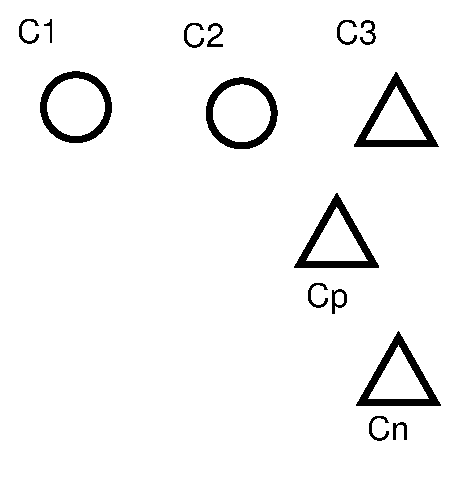
\includegraphics[width=120pt]{./Drawn/FlipPrecedence}
\caption{Example of a Flip/Shunt Scenario.}
\label{fig:flipprecedence}
\end{figure}

The resultant `change' to the case-base for $Cp$:
\begin{itemize}
	\item Added: 
	\begin{itemize}
		\item $ReachabilitySet(Cn)~=~\{C3,~Cp\}$
	\end{itemize}
	\item Removed:
	\begin{itemize}
		\item $DissimilaritySet(Cn)~=~\{C1,~C2\}$
	\end{itemize}
\end{itemize}

From this information alone, we cannot infer which of $C1$ and $C2$ was shunted (or even that anything was shunted if we don't know $k$). To minimize the information requirements that this algorithm carries, we thus decide to consider $C1$ and $C2$ as flip-related changes.

\subsubsection{Inferring the changes of coverage / liability from reachability / dissimilarity}
The duality property as described in Section \ref{sec:duality} allows us just to consider reachability and dissimilarity changes, and infer coverage and liability changes respectively. Reachability and dissimilarity are chosen due to easier reasoning about programatically, since they deal with NNs as opposed to rNNs.

The operation \verb!PlaceDuals(CPs)! represents iterating through a given Change set, and for each reachability / dissimilarity related change, adding the corresponding duality set change (coverage / liability).

\subsection{Counting Shunts}
If a shunt related remove happens, it will happen for \emph{every} possible label with no exception. This duplication holds no benefit for final weighting, since shunts would be counted for each of the number of labels there are. We therefore decided to only total shunts for a single label.

\subsection{Counting Flips}
If there are more than 2 labels and we totalled across different labels, both flip directions \emph{might} lead to multiple-counting, depending on the exact cause of the flip. A flip may occur for some, or all of the supposed labels.

We do not attempt to count unique instances here, as the weighting attached due to the duplicates is somewhat useful. If a flip occurs for e.g. 3 out of 4 labels for a case, it is somewhat more relevant than if it occurs for 1 of the 4 labels.


\section{A Grammar for Naming Competence Strategies}

Due to the availability of compute resources with the incorporation of cluster-like functionality in the platform developed, it was possible to execute a large quantity of competence-based selection strategies. Naming individually every single strategy would be unwieldy at best, therefore a naming convention was adopted based on the various decision points in the strategies we developed.

\subsection{Decision Points}

\subsubsection{Locality}
\emph{Locality}, in the context of our selection strategies, indicates which cases' RCDL sets we consider during the selection among the candidate cases.

\emph{Local} refers to just the candidate case's RCDL sets being considered, while \emph{Global} relates to the candidate case's effects on the RCDL sets of the cases already in the case-base. 

While there certainly is overlap due to the duality property, it is also possible that other cases not directly related to the candidate case can be affected due to the candidate case's addition. Some of these side-effects, in particular what we term `flips', can be quite interesting.

\subsubsection{Cross Label Aggregation}
RCDL profiles are highly dependent on knowing the labels of the cases in question. Given that we do not know what the label of a candidate case will be before we provide it to the oracle, it is necessary to consider ``what-if'' style analysis when considering the RCDL effects of a candidate case.

For the purpose of combining the possible labels' measures, we chose two basic aggregation approaches: 
\begin{enumerate}
\item \underline{Total:} 

Simply adding the overall measure values produced for each of the labels.
\item \underline{Deviation:} 

Calculating the standard deviation between the values of the different possible labels.
\end{enumerate}

\subsubsection{Quantity Goal}
The overall goal of the strategies we developed is based on \emph{minimizing} or \emph{maximizing} the scores of the individual cases.

\subsubsection{Density Inclusion}
Density information regarding the dataset can also be incorporated as a measure in the overall strategy. The density measure is defined as the average similarity to all other cases in the entire dataset, stretched to the range 0 to 1. The sparsity of a case we simply define as 1 minus the density of the case.

When either measure is included, it is combined with each RCDL measure in a non-weighted average fashion.

\subsubsection{Set to Scores Mapper}
The set to scores mapper defines the mechanism to map a single R, C, D or L set for a single case, to a sequence of scores. This may not necessarily be a one-to-one mapping for the cases contained in the set.

We define 4 simple maps:

\begin{enumerate}
\item \underline{All-Pairs Similarity (incl source):} 

This maps a set to the similarity values for the all-pairs of the set plus the source case from which the set emanates.
\item \underline{All-Pairs Similarity (excl source):} 

This is similar to the previous mapper, except it does not include the source case from which the set emanates.

\item \underline{Direct Similarity:} 

This maps a set to the similarity values between the source case and each case in the set in question.

\item \underline{Counting:} 

This simply maps a set to a sequence of ones of length equal to the size of the set.
\end{enumerate}

\subsubsection{Set Scores Reducer}
The reducer here combines a set of scores down to a single score. Two simple reducers are defined; total, and average.

\subsubsection{RCDL Sets to Use}
Another decision point for a strategy is which of the RCDL sets to consider in the strategy. For our strategies, for a given strategy, the other decision points applied to one set are also applied separately to the others. The same decision points are used for each of the RCDL sets in the strategy. 

It should be noted that this grammar design does not allow representation of a selection strategy with more than one RCDL set, but based on different measures, but is sufficient for us given that we only experimented with basic hybrid strategies. 

\subsubsection{Measures Reducer}
The individual RCDL measures for a strategy need to be combined in some fashion. We chose simple summing, this being equivalent to non-weighed average given that the denominator is the same for every candidate, and given that no more combinations are done subsequent to this last step. We represent this simply as `+'. The other possibility considered was multiplication, but we decided against this due to the issue with how to deal with zero values, but in our naming convention, would be represented with `*'.

\subsection{Decision Points Summary}
\begin{tabular}{|l|l|x{200px}|c|}
\hline 
ID & Decision Point & Possible Values & \# Values\tabularnewline
\hline 
\hline 
1 & Locality & Local, Global & 2\tabularnewline
\hline 
2 & RCDL Sets & \{Reachability\}, \{Dissimilarity\} . . . \{Reachability, Coverage\},
\{Reachability, Dissimilarity\} . . . & 17\tabularnewline
\hline 
3 & Measure Reducer & +, {*} & 2\tabularnewline
\hline 
4 & Set Scores Reducer & Average, Total & 2\tabularnewline
\hline 
5 & Set to Scores Mapper & All Pairs Similarity (incl source), All Pairs Similarity (excl source),
Direct Similarity, Counting & 4\tabularnewline
\hline 
6 & Density Inclusion & With Density, With Sparsity, (None) & 3\tabularnewline
\hline 
7 & Cross Label Aggregator & Total, Deviation & 2\tabularnewline
\hline 
8 & Quantity Goal & Minimization, Maximization & 2\tabularnewline
\hline 
\end{tabular}

\subsection{Combining Decision Points to a Name}
Decision points are used to generate a string as follows, where `[ID]' represents the value of the decision point referenced by `ID' in the matrix above:

\begin{quote}
[1] ([2] with items separated by [3]) [4] [5] [6] Cross-Label [7] [8]
\end{quote}

\subsection{Example Strategy Name}
For this example, we shall consider:
\begin{quote}
Local Liability + Coverage Total Counting (With Sparsity) Cross-Label Total Minimization
\end{quote}

The decision points are then extracted as follows:

\begin{tabular}{|l|l|c|c|}
\hline 
ID & Decision Point & Value\tabularnewline
\hline 
\hline 
1 & Locality & Local \tabularnewline
\hline 
2 & RCDL Sets & Liability, Coverage \tabularnewline
\hline 
3 & Measure Reducer & + \tabularnewline
\hline 
4 & Set Scores Reducer & Total \tabularnewline
\hline 
5 & Set to Scores Mapper & Counting \tabularnewline
\hline 
6 & Density Inclusion & With Sparsity \tabularnewline
\hline 
7 & Cross Label Aggregator & Total \tabularnewline
\hline 
8 & Quantity Goal & Minimization \tabularnewline
\hline 
\end{tabular}

Stepping through each in turn:

\begin{enumerate}
	\item \underline{Locality: Local}
	
	Just the RCDL sets of the candidate case are considered.
	\item \underline{RCDL Sets: Liability, Coverage}
	
	The measure subsequently defined shall be calculated separately for each of the liability and coverage sets of the candidate case.
	\item \underline{Measure Reducer: +}
	
	The value for the liability based measure and the value for the coverage based measure will be 
	combined through simple summing.
	\item \underline{Set Scores Reducer: Total}
	\item \underline{Set to Scores Mapper: Counting}
	
	The sequence of values generated through the mapper (counting) will be reduced by totalling. In this strategy, this is simply the cardinality of the RCDL set in question. This will be used as the overall score for that set.	
	\item \underline{Density Inclusion: With Sparsity}
	
	Density information shall be incorporated through the notion of sparsity, with sparsity combined with each RCDL based measure through non-weighted average.
	\item \underline{Cross Label Aggregator: Total}
	
	A score will be calculated for each possible label, with the scores combined to an overall score through simple summing 
	\item \underline{Quantity Goal: Minimization}
	
	The overall goal of the strategy will be minimization. This means that for each candidate set, a value will be assigned by the strategy, and the candidate set with the lowest value will be selected (with random tie breaking used in the case of ties for lowest).
	
\end{enumerate}

\section{Selection Strategies}

\subsection{Simple Single-Set Counting Strategies}

\subsubsection{Local Reachability (Counting)\label{sec:compstrat1}}
When Supposing a single case for addition to the case-base, irrespective of the label we choose to suppose, the case-base will classify it with only one label. For example, in Figure \ref{fig:NNsCorrect}, irrespective of if we suppose Cn to be a triangle, or a circle, the case-base will still classify it a circle. Thus, the reachability set of Cn will only get populated in one instance - when we suppose Cn to be the same label as the case-base classifies it.

This holds true in Supposing any case for the case-base. A supposed case will only have its reachability set populated for one single label for a case-base state - the label that the case-base classifies it as. Assuming a non-empty case-base, for when the reachability set is populated - the cardinality of the set will always be between 1 and k.

With the absence of further knowledge, we could guess that when the reachability set for a new case is small compared to other candidate cases, the case-base is relatively uncertain about the new case. As a result, by choosing a new case from the unlabelled set which results in a minimally sized reachability set for that new case, we get a basic form of uncertainty sampling\footnote{If we were using non-weighted voting in our KNN implementation, we would get exactly uncertainty sampling. With distance weighted voting, it's not quite the same, since our basic strategy simply takes only the cardinality of the reachability set into account, and not the distances of the cases within it.}.

This strategy takes this approach exactly - assigning an overall score to each unlabelled case equal to the total of the reachability set supposes across all the different possible labels\footnote{Totalling is sufficient because we are guaranteed that the reachability set will be empty for all but one of the supposes. So totalling is equivalent to just taking the value of the non-empty reachability set.}. The unlabelled case with the minimum score is then selected. Ties are broken at random.

\subsubsection{Local Coverage (Counting)}

The intuition around this strategy is that by trying to find unlabelled cases which have a roughly equal positive effect for the different possible labels, we get cases which are close to classification boundaries.

\begin{figure}[h!] \centering
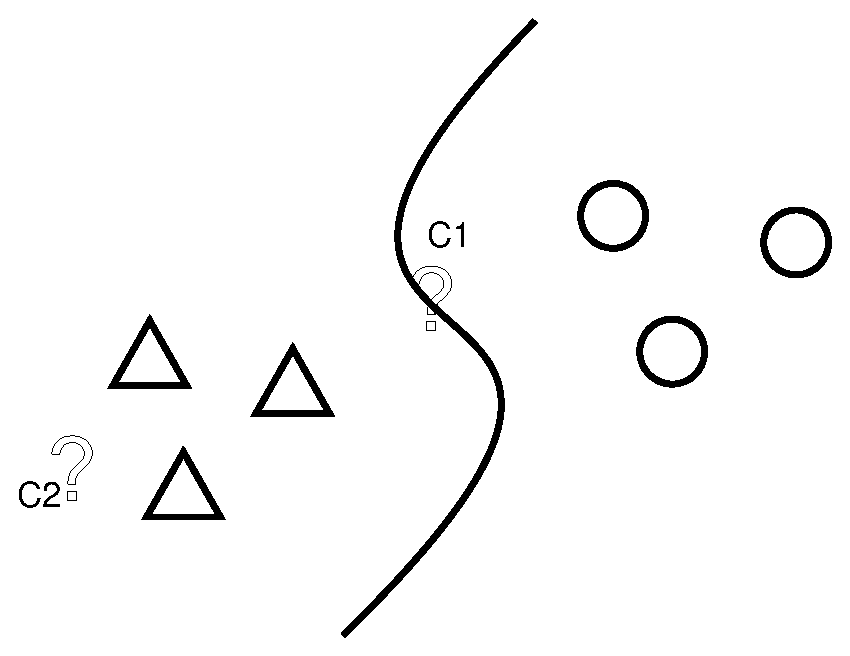
\includegraphics[width=200pt]{./Drawn/NCADMin}
\caption{Example of classification boundary for 2 areas (Triangle and Circle), with two candidate cases for selection, C1 and C2.}
\label{fig:ncadmin}
\end{figure}

In the example presented in Figure \ref{fig:ncadmin}, k=4, and we have two candidate unlabelled cases C1 and C2. With the case-base as it stands, the classification boundary we can guess is in the middle of the circle and triangle regions (denoted by the line).
 
Intuitively - if we knew the value of C1, it would better tell us where the classification boundary should be. If it turned out to be a circle, it would push the classification boundary left towards the triangles. Similarly, if it turned out to be a triangle, it would push the classification boundary right towards the circles. 

C2 would be less useful to retrieve a label for, since compared to C1, we know more about the region in which it lies.

If we were to look at the size of the coverage sets of C1 and C2 for the different possible classifications:

\begin{tabular}{|c|c|c|c|}
\cline{2-4} 
\multicolumn{1}{c|}{} & Coverage if Triangle & Coverage if Circle & Standard Deviation\tabularnewline
\hline 
C1 & 3 & 3 & 0\tabularnewline
\hline 
C2 & 3 & 0 & 2.12\tabularnewline
\hline 
\end{tabular}

\vspace{10pt}

This strategy chooses the case with the minimum Standard Deviation between the possible labels, with random tie-breaking used.

One thing that initially falls out of this strategy is that, during the early selections, it will likely choose relatively diverse cases. Unlabelled cases which have no rNNs in the case-base will have empty coverage sets irrespective of their supposed label, and thus, a standard deviation of 0.

After all of the diverse cases have been selected, it will then move onto balancing more similar to as described in the example above.


\subsubsection{Local Dissimilarity (Counting)}
\begin{figure}[h!] \centering
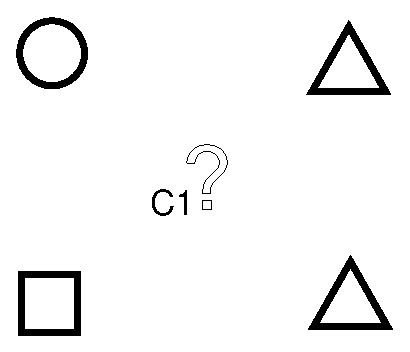
\includegraphics[width=100pt]{./Drawn/NDATMin}
\caption{Example of unlabelled case relative to its k-nearest-neighbours within the case-base.}
\label{fig:ndatmin}
\end{figure}

In the example presented in Figure \ref{fig:ndatmin}, case $C1$ is an unlabelled example being supposed, with $k=4$. Three labels are shown, Square, Circle and Triangle - but a fourth is also present in the dataset - an X. $C1$ will be classified as a Triangle by the case-base. 

If we consider the dissimilarity set of the new case for the different supposes, we concentrate on the other cases which contribute to its incorrect classification. We get the following table:

\vspace{10pt}
\begin{tabular}{|c|c|x{150pt}|}
\hline 
Supposed Label & Dissimilarity Set & Description\tabularnewline
\hline 
Triangle & \{\} & If it's a Triangle, then it is correctly classified by the case-base,
and so won't have a Dissimilarity set.\tabularnewline
\hline 
Square & \{Triangle, Triangle, Circle\} & Incorrectly classified. The Square isn't aiding in the misclassification,
so it's only the remaining NNs.\tabularnewline
\hline 
Circle & \{Triangle, Triangle, Square\} & Incorrectly classified similar to above. Circle isn't aiding, so just
the remaining NNs.\tabularnewline
\hline 
X & \{Triangle, Triangle, Circle, Square\} & Incorrectly classified. All the NNs are contributors.\tabularnewline
\hline 
\end{tabular}

\vspace{10pt}

If we use $C_{P}$ to denote the set of cases in the NNs of $C1$ where the case is of the same label as the case-base's classification of $C1$, and $C_{N}$ to denote the set of cases in the NNs with a different label. Let $L$ denote the set of possible labels. In the above example $L=\left\lbrace Circle, Triangle, Square, X\right\rbrace$.

Each element in $C_{P}$ will be appear in each suppose except for:
\begin{enumerate}
	\item The suppose of the label the case $C1$ is classified as.
\end{enumerate}

Somewhat similarly, each element in $C_{N}$ will appear in each suppose except for:
\begin{enumerate}
	\item The suppose of the label the case $C1$ is classified as.
	\item The suppose of the label equal to the $C_{N}$ element's label.
\end{enumerate}

From this, we can derive the formula for the total (summed sizes) of the dissimilarity sets in terms of the contributions of $C_{P}$ and $C_{N}$:
\[ Total= (|L| - 2)\times |C_{N}| +(|L| - 1)\times |C_{P}|  \] 

We can represent $|C_{P}|$ in terms of $C_{N}$:
\[ |C_{P}| = k -  |C_{N}| \]
where $k$ is the length of the NNs set (essentially a constant for the current state of the case-base). Incorporating this with the previous equation, we get:
\begin{align*}
Total &= (|L| - 2)\times |C_{N}| +(|L| - 1)\times (k - |C_{N}|) \\
&= |L| \times |C_{N}| - 2\times|C_{N}| + |L|\times k - |L| \times |C_{N}| - k + |C_{N}| \\
&= (|L| - 1) \times k - |C_{N}| \\
\end{align*} 

The $ (|L| - 1) \times k $ part will be a constant for a single case-base state. $|C_{N}|$ represents the number of disagreeing neighbours. A high number of disagreeing neighbours would indicate that the case-base is relatively uncertain about the classification. Thus - a strategy to semi-emulate uncertainty sampling (though in a less fine-grained manner) is to maximize $|C_{N}|$. To do this, we should minimize $Total$.

\subsubsection{Local Liability (Counting)}
There are two types of cases which can appear in the new case's liability set:
\begin{enumerate}
	\item A case which was already misclassified, and the new case simply joins in in the misclassification.
	\item A case which has enough sway with an existing case to cause the case to go from correctly classified, to incorrectly classified.
\end{enumerate}

In each, the new case is somehow aiding in the incorrect classification of an existing case in the case-base. If we forget about the possibility of mislabelled data, the intuition is that this is generally a bad thing - we are `overpowering' a neighbourhood of the case-base with data which could cause mislabelling.

Totalling here, as in other strategies, is probably not the best approach - but as a simplistic initial investigatory strategy, we try to minimize the total of the new case's liability set summed over the different possible supposes.

\subsection{Pruned Cross Product Strategies}
Understandably, given the 6,528 strategies possible through the simple cross-product grammar based approach presented, it was necessary to prune the combinations to a more tractable level. As such - the following restrictions on decision point combinations were made:

\begin{itemize}
	\item \underline{No Global Strategies:}
	
	Global strategies require more careful thought than local strategies given the possibility of shunting and flipping, and dealing with many cases' sets as opposed to just the candidate case. Certain measures, such as all-pairs similarity, also would need tweaking. As a result, we decided not to include global strategies in our simple cross-product style investigation.
    \item \underline{Only Minimization Strategies:}
    
    Strategies which were initially thought out were all minimization strategies to try to encourage some kind of diversity. To cut down largely the number of possibilities given the somewhat limited compute-time available, we only chose minimization cross-product based strategies.
    \item \underline{Disallow Averaged Counting}
    
    Averaging makes sense for the similarity based set scores, but for counting, it would lead to more of a boolean 0 or 1 defining if the set was empty or not. While this might well lead to valid strategies in some cases, we wanted to reason more about the contents of the sets as opposed to simply if they contained elements or not. 
    \item \underline{Use Sparsity as the only density based measure:}
    
    Due to our decision to only do minimization strategies, we do not use density in our measures, since we want to pick from dense regions, thus minimize sparsity.
    \item \underline{Exclude Dissimilarity:}
    
    From initial investigation, it was noted that our simple dissimilarity strategies performed identically or near-identically to the corresponding reachability strategies. This is relatively unsurprising given the definition of dissimilarity, and given that we perform the calculation for each possible label, with each getting equal weighting.
    \item \underline{Restrict hybrid strategies to well performing single-set strategies:}
    
    Hybrid strategies are a large reason for the high number of cross-product based strategies. We thus limit our hybrid strategies (the strategies with more than one RCDL set considered) to a small selection of well-performing single-set strategies. The strategies we picked:
    \begin{itemize}
        \item Total Direct Similarity (With Sparsity) Cross-Label Total Minimization
        \item Total All-Pairs Similarity (incl source) (With Sparsity) Cross-Label Deviation Minimization
        \item Total Counting (With Sparsity) Cross-Label Total Minimization
        \item Total Counting Cross-Label Total Minimization
    \end{itemize}
\end{itemize}

These restrictions lead to a somewhat more manageable total of 100 cross-product based strategies.

\subsection{Global Counting-Based Strategies}

\subsubsection{Global Coverage (Counting)}

\paragraph{Direct}

The direct rNN's coverage added is equivalent to the new case's reachability added. See Section \ref{sec:compstrat1} for justification on minimization.

\paragraph{Shunted}

When a case is shunted from an NNs set by the new case, its coverage set size might be reduced by one (i.e. a coverage set removal). Many such removals (at least in the situation of a relatively populated case-base) would indicate that the new case is making an area more dense.

\paragraph{Flip}

If the new case causes a `flip' in the correct-classification-status of an rNN, that rNN's other NNs may have gained or lost (or neither) items in their coverage sets. The desire would be to minimize flips to incorrect classifications (Flip related coverage removals), but increase flips to correct classification (Flip related coverage additions).

Because the overall aim in the strategy is `minimization', to give positive contribution to Flip related coverage additions, and negative contribution to Flip related coverage removals, we subtract Flip related coverage additions, and add Flip related coverage removals.

\paragraph{Overall Formula}
\[  
  T~=~Direct_{C+}~+~Shunted_{C-}~-~Flip_{C+}~+~Flip_{C-}
\]

This value is computed for each candidate case, summed across the possible labels. The candidate case with the minimum value is selected.

\subsubsection{Global Reachability (Counting)}
\paragraph{Direct}
A high number of additions to Direct reachability sets of Other cases would indicate that the new case is in a relatively dense region. To attempt to increase the diversity of new cases, we would thus like to minimize this.

\paragraph{Shunted}
Shunting a `helping' neighbour for an existing case could be considered a bad thing, since we are moving in a neighbour for which an existing neighbour was already covering that space. We would like to minimize these.

\paragraph{Flip}
Causing a flip to correctly classified is a positive thing (Flip related reachability additions), whereas causing a flip to incorrectly classified a bad (Flip related reachability removals).

\paragraph{Overall Formula}
\[  
  T~=~Direct_{R+}~+~Shunted_{R-}~+~Flip_{R-}~-~Flip_{R+}
\]

We would like to minimize this value overall.

\subsubsection{Global Liability (Counting)}
\paragraph{Direct}
(No real point considering this with the whole double counting that cropped up in CompStrat 4.)

\paragraph{Shunted}
Causing a `shunt' of a hurtful case could be considered a positive action. The added case that caused the shunt will hopefully add more information regarding that area of the case space. 

\paragraph{Flip}
Causing a case to flip to incorrectly classified would lead to flip related liability additions, whereas causing a flip to correctly classified would lead to flip related liability removals. We would like to minimize flips to incorrectly classified, while maximizing flips to correctly classified.

\paragraph{Overall Formula}
\[  
  T~=~Shunted_{L-}~+~Flip_{L-}~-~Flip_{L+}
\]

This value is computed for each candidate case, summed across the possible labels. The candidate case with the maximum value is selected.

\subsubsection{Global Dissimilarity (Counting)}

\paragraph{Direct}
A high number of additions to Direct dissimilarity sets of Other cases would indicate that the new case is in a relatively dense region. To attempt to increase the diversity of new cases, we would thus like to minimize this.

\paragraph{Shunted}
To also aid in identifying diverse cases, we minimize the shunted neighbours here.

\paragraph{Flip}
Causing a flip to correct classification (Flip related dissimilarity removals) could be construed as positive, whereas flips to incorrect classification (Flip related dissimilarity additions) as negative.

\paragraph{Overall Formula}
\[  
  T~=~Direct_{D+}~+~Shunted_{D-}~+~Flip_{D+}~-~Flip_{D-}
\]

\subsection{Global Similarity-Based Strategies}
We also briefly experimented with global similarity-based strategies. We used direct similarity instead of counting, and applied the same formulas as defined for the global counting-based strategies, with the exceptions that for coverage and reachability, we subtract instead of add shunted.

\chapter{Experimental Analysis\label{cha:expanalysis}}
\section{Datasets Used}

\DTLloaddb{non_textual_data_stats}{./ExperimentResults/all_non_textual_data_stats.csv}
\DTLloaddb{textual_data_stats}{./ExperimentResults/all_textual_data_stats.csv}

\subsubsection{Non-Textual}
\DTLdisplaylongdb{non_textual_data_stats}

\subsubsection{Textual}
\DTLdisplaylongdb{textual_data_stats}

\section{Results}
Due to the large quantity of datasets experimented on, along with the sheer volume of selection strategies attempted, we do not present the results in entirety here. The reader can view these in the appendix, in Section \ref{sec:fullresults}.

In each category, we choose a small subset of the noteworthy results, comparing against against some previously presented well-performing strategy to aid in comparison.

\newpage

\begin{python}
from collections import OrderedDict
from utils import printFigure
d = OrderedDict()
d['Baseline Comparison'] = "./ExperimentResults/selected_baseline/"
d['Competence Based Counting'] = "./ExperimentResults/selected_competence_counting/"
d['Competence with Similarity'] = "./ExperimentResults/selected_competence_with_similarity/"
d['Basic Density Incorporation'] = "./ExperimentResults/selected_sparsity/"
d['Competence with Sparsity'] = "./ExperimentResults/selected_competence_with_sparsity/"
d['Competence Set Hybrids'] = "./ExperimentResults/selected_competence_hybrids/"
for (n, d) in d.iteritems():
    print r'\subsection{%s}' % n
    print r'\vspace{15pt}'
    printFigure(d)
\end{python}

\section{Results Summary}
\DTLloaddb{presented_summary}{./ExperimentResults/selected_all_presented/summary.csv}
\resizebox{\textwidth}{!} {
  \DTLdisplaydb{presented_summary}
}

\section{Results Discussions}
It should be noted that the following discussion also incorporates the full results, as opposed to the small subset presented above.

\subsection{Random Selection Performance}
It bears mention that, considering how utterly inexpensive a strategy it is, random selection performs quite well. 

\subsection{Local Reachability Counting}
Considering their simplicity, strategies involving local reachability counting perform very well compared to uncertainty and random sampling. 

One possible reason for this is due to the strategies' benefit of creating a candidate set of relatively uncertain cases from which random selection is used. This is slightly different to uncertainty sampling based on non-weighted voting, in that firstly, voting is performed in a distance weighted fashion to determine the probable label, then the cardinality of the set of cases in the k-nearest neighbours with the same label is minimized.

In this way, it doesn't fall prey to the traditional downfall of pure uncertainty sampling of always querying outliers, instead picking from the relatively uncertain cases at random.

\subsection{Benefit of addition of Sparsity}

The addition of density information (in the form of sparsity), has an undeniable benefit to the competence-based strategies, especially on textual data. The benefit is less seen on the non-textual data, probably due to the quicker convergence and smaller data sizes.

It should be noted that Diversity + Sparsity, and Uncertainty + Sparsity, also do quite well. We decided to perform basic tests on these to determine if the increase in competence strategies' performance was at all significant. The competence strategies on their own generally aim to pick somewhat diverse cases, and thus adding density information intends to augment this diversity picking with information regarding density of that region in the dataset.

Some of the competence strategies augmented with sparsity do perform significantly better than either Diversity + Sparsity, or Uncertainty + Sparsity, on the textual datasets. Though given the naive approach used for these two comparative strategies, further work is needed to compare with established strategies which aim to incorporate uncertainty, density, and diversity.

\subsection{Deviation almost equivalent results to total}
Although deviation and totalling are technically different approaches, for the datasets tested and the manner in which we used these approaches in our selection strategies, they produced for the most part identical performance.

\subsection{Poor hybrid results}
Upon consultation of the full results, and as demonstrated in the subset of the results above, it can be seen that the hybrid strategies in our simple combinations appear to be dominated by one of the sets, being identical to that one set's non-hybrid strategy. 

\chapter{Conclusions and Future Work\label{cha:conclusions}}

\section{Project Results}
The project has led to some promising competence-based selection strategies which perform quite well compared to traditional strategies. While the results vary between datasets, there being no single overall winner, they do prove somewhat that incorporating competence in active learning, as opposed to its traditional domain of case-base maintenance, might have some merit. Though certainly, further work would be needed to establish this more concretely.

\section{Contributions Made}
\subsection{Experimental Platform}
The Python-based platform developed for the project has some useful features for selection-strategy experimentation in a pool-based active learning context.

It allows pluggable definitions of selection strategies, without requiring code changes to the main platform. It also has very pluggable definitions for things like the oracle, stopping condition, classifier, etc. It could thus be used for evaluations far beyond the current scope of this project.

One small but useful additional capability of the platform is how it deals with data loading and distance computation. It provides two interoperable formats to store pre-computed distance information along with the data. This allows for very different platforms to be used in initially processing the data. Even in this project, it allowed textual data to be added by using the facilities of SciKit Learn, but required no modification to the platform code.

The experimental result re-use mechanism is another useful feature to the platform, which allows it to read in previous results, and use them if necessary when running the new experiment. 

The capability of the platform to operate on a distributed cluster-based map-reduce fashion is another significant, albeit a relatively undocumented benefit given the late stage of the project that the feature was added. 

\subsection{Incremental Algorithm to RCDL}

The incremental algorithm to RCDL profile generation presented in Section \ref{sec:incrstrategy} is a new addition to the area. It was not necessary in \citet{Delany2009} due to how she was using it, but for active learning approaches, having an incremental approach becomes a lot more relevant. 

The `suppose' operation is also somewhat novel, allowing selection strategies to determine in advance what the changes to the RCDL profiles would be if it picked a certain case, and that case turned out to have a certain label.

\subsection{Competence Based Selection Strategies}

We presented how we interpret the changes that might occur the competence profiles of cases following the addition of a new case to the case-base, and ran experimentation to test our derivations.

While the presented competence based strategies were by no means ground-breaking in their results, I believe their investigation still contributed useful thought-experiments in the field, and also set some of the ground work for potential future investigation into competence based methodologies.

\subsection{SciKit-Learn Fix Contribution}

Although relatively trivial in size, I identified a bug in the SciKit-Learn 20 newsgroups textual data loading mechanism. I fixed the bug, added unit tests to verify the presence of the bug, and the fix written, and subsequently pushed the changes back to the main SciKit-Learn repository. The community members in charge of the repository verified and accepted the change.


\section{Further Research Opportunities}
\subsection{Statistical Analysis of Suppose Change Distribution}
In our research, we treated the selection strategies and overall experimentation as simple black boxes. We would try implementing various strategies, run the experiments with the new strategies, and simply look at the outputted results, comparing them to those of previous strategies.

At no stage did we actually analyse the individual choices that the strategies made for the purposes of understanding the results or improving the strategies. While much scope exists for more in depth analysis, at a very minimum, one interesting area for future work would be to perform statistical analysis on supposes for multiple datasets to better understand distribution of types of case profile changes.

When we were selecting minimums, I am curious as to the level of zeroes present, whether for some of the strategies on certain datasets, they were almost equivalent in behaviour to random sampling. I also think it would be useful for when developing new strategies as to the frequency and size of the different types of RCDL changes from the selection of a case.

As a result of all this, I believe there would definitely be benefit in spending the time to perform statistical analysis on suppose operation based changes.

\subsection{Try more sophisticated RCDL-augmented selection strategies}

The work we did on building RCDL based selection-strategies was somewhat exploratory, focussing mainly on just the RCDL concepts. It would be interesting to try more sophisticated techniques in using RCDL profiles, by augmenting some existing selection strategies, both established and novel.

It might also be interesting to go in the other direction - to try to incorporate concepts from existing strategies into the simple RCDL based strategies we defined, for example taking into account case uncertainty and label probability when doing the suppose operations.

\subsection{Use `suppose' approach in developing case-base maintenance algorithms}

\citet{Delany2009} investigated case-base maintenance algorithms using RCDL profiles in a compute-once fashion, generating the profiles at the outset of the algorithm and subsequently just using this snapshot for the remainder of the algorithm.

It would be interesting to try using an incremental  ``suppose'' approach similar to what we developed in investigating case-base maintenance algorithms.

\subsection{Improve Visualization Capabilities}

The visualization capabilities described in Section \ref{sec:selectiongraphs} were a two day effort in removing some of the `black-box' nature of our experimentation approach. This feature has scope for massive improvements:

\begin{itemize}
	\item \textbf{Provide dynamic interactive view with overlay information}:
	
	      Currently, only a static output is produced following the experiment. I believe it would be useful to have a more dynamic output option which includes the ability for user interaction, providing for example:
	      \begin{itemize}
	      	\item Overlay information about the relevant cases
	      	\item Information regarding the state of the case-base
	      	\item The decision process surrounding the current 
	      \end{itemize} 
	\item \textbf{Allow querying the engine}:
	
	      As opposed to just viewing information regarding the current state of the experiment, it would be useful to be able to perform queries against the engine such as ``What effects would selecting this case from the unlabelled set?''. It could also be useful to actually have input into the experiment by being able to actually force the selection of a case to see the consequences as the experiment continues running.
\end{itemize}

I believe that by researching and implementing a generic visualization feature for the platform, the task of selection-strategy research and development would be eased by allowing greater visibility into the decisions of selection strategies.

The reason I would count this as a research opportunity as opposed to pure development is that  investigation around how to effectively convey information, and provide interactivity to the user would need to be carried out.

\subsection{Try alteration on definition of Delany's `Contributes' notion}

Delany's definition of `contribution' is as one would expect for binary classification, but I feel is somewhat counter intuitive for her `negative' sets (liability and dissimilarity) when performing multi-label classification.

If a case is mislabelled by the case-base, she defines a case contributing to that misclassification as any neighbour in the k-nearest neighbours of the original case that have a different label to the label of the original case. 

In the example presented in Figure \ref{fig:equaldistancemisclassifieseg}, even though $C1$ plays no role in the classification of $X$, by Delany's definition, it still contributes to the incorrect classification, and thus $Misclassifies(X,~C1)$. This has implications in the liability and dissimilarity sets of $C1$ and $X$ respectively. 

I believe however that it would be more intuitive if we defined contribution towards classification as the neighbours in a case's k-nearest neighbours that have the same label as the classification of the case.

\subsection{Maintain information about `helping' and `hindering' sets}
A case either has a reachability set, or dissimilarity set - never both. This either-or nature is convenient for Delany's binary-style analysis, but throws away all information about the \emph{competing} set (be it reachability, or dissimilarity).

For example, in Figure \ref{fig:NNsCorrect}:
\begin{itemize}
	\item $reachability(Cn)=\left\{C1,~C2\right\} $
	\item $dissimilarity(Cn)=\left\{ \right\} $
\end{itemize}

Here, no knowledge of $C3$ is maintained. I believe it might be useful to also maintain additional sets `helping' and `hindering', along with their duals.

\subsection{Reconsider Liability Strategies}
The liability-based strategies perform quite poorly overall. Some further consideration and investigation is deserved around the causes.

\subsection{Try more hybrid strategies}
Our investigation into hybrid RCDL set strategies was very limited. Considering different combinations in a more meaningful and systematic way could prove interesting.

\subsection{Incorporate certain aspects of global strategies}
Certain global-type changes, in particular `flips', are quite interesting, and much underused in our work. Selective incorporation of side-effect style information could allow some interesting variations on some of the strategies we defined, and also more traditional strategies.

\subsection{Profile datasets, applying appropriate strategies}
Analysis on which strategies perform well based on dataset characteristics could be useful. Certain types of strategies perform very well on some datasets, but only mediocre on others. For example, sparsity based strategies perform well on the textual data.

Trying to dynamically pick which strategy to apply based on the current case-base, and the dataset in general might be promising.

\section{Platform Development Opportunities}

\subsection{Improve Test Coverage}

Test coverage of the platform, and experimentation in general, was relatively low. For certain core operations, such as classification and incremental profile building, unit tests were written, but large portions of the overall code have not been methodically tested. 

If the platform were to be used in a more intense fashion, increasing the test coverage should be a work item.

\subsection{Document and package platform for general release}

Given the one-person nature of the development of the platform, along with the focus on the research and results of selection strategies, the code of the platform is severely lacking in documentation. 

To be more usable as a general purpose platform that others could easily also use, it would be good to properly document the code, and restructure the code to a more disciplined package. 

\subsection{Change to support other types of case-based reasoning experimentation}

The current platform was developed for the sole purpose of investigating selection strategies in the context of pool-based active learning. A lot of the code however would also be applicable if one were performing other types of case-based reasoning research.

At a minimum, it would be nice if basic support was added for other core scenarios, such as case-base maintenance. This would allow researchers to build on top of this the elements that are unique to their investigations.

\section{Closing Thoughts}
\subsection{Backing Source Code should follow publications}
I believe that, at a minimum for any public funded research, a link to backing source code should be a requirement for any publications produced. I find it baffling that results can be presented without any capability for reproducing the experiment. It feels contra to the general purpose of public research.

It is possible that small bugs in people's code could invalidate entire experiments. Understandably, there would be fear when releasing source code as a result, but the work feels somewhat pointless otherwise. This is assuming good intention, but there is also the fact that researchers can carefully choose which results to publish, ignoring all the failed results.

Not only would the requirement of source code provision aid in preventing the above, it would also better encourage re-use and collaboration among researchers of similar areas.

\subsection{Usefulness of active learning and case-based reasoning}

The project has opened my eyes somewhat to the benefit of active learning. In particular, the fact that the concepts apply beyond traditional domains like text analysis, and into more modern ones like recommendation engines.

I don't think active learning is the `next-big-thing', but the concepts in it are undeniably useful, and it's an area that I believe active research  will continue to be beneficial. I will be especially interested in seeing in the coming years the new areas in which the concepts get successfully applied to.

\subsection{Novelty of Competence Models}

The notion of competence models appears to be a relatively unexplored area in case-based reasoning. The profiling of individual cases based on their competence-contributions to a case-base provides a different mindset from which to approach the domain.

Somewhat pessimistically, I don't believe competence oriented research alone will suddenly solve all the woes of active learning, or general case-based reasoning. I do however think it is a useful addition to the general toolbox of techniques within the case-based reasoning community, and I'm shamelessly glad to have contributed ever-so slightly to it.

\chapter{Appendix}
\section{Project Source Code}
This Project's source code has been placed online \citep{web:projectsourcecode}. Aside from the aim for this project to be as Open Source as possible, it is my strong belief that any research which actually aims to advance a given field should have all the things required to reproduce the results publicly available without having to make explicit requests to the authors. 

It surprises me the massive body of research that doesn't follow this methodology - especially research which is publicly funded. It is important that external parties have full opportunities to validate experiment results. Small bugs in programs may cause entire projects to have invalid (though convincing) results, and while this would be disastrous for the researchers involved to have these discovered publicly, it is necessary for the actual progression of scientific knowledge.

By having all backing materials available, it also allows other researchers to continue with the original research, as opposed to starting from scratch and re-developing all the architecture necessary again and again.

\section{Full Experiment Results Listing\label{sec:fullresults}}
Due to the incorporation of a map-reduce framework towards the end of the project, along with scripts to execute across several hundred college computers, throughput was available to run many additional experiments. Due to the limited quantity of time remaining at the time, a `dumb' cross-product methodology was used to generate experiments based on the methods used previously. 

Only a small proportion of these new generated experiments were some way promising, but for completeness, the full listing of experiments along with their results are presented here. Due to the cross-product style strategy name length, these names have been abbreviated, but due to their resulting unintelligibleness, the reader is recommended to instead consult the results online \cite{web:projectsourcecode}.

\begin{landscape}
\subsection{Non-Textual}
\DTLloaddb{all_non_textual_summary}{./ExperimentResults/all_non_textual/summary_abbreviated.csv}
{\scriptsize \DTLdisplaylongdb{all_non_textual_summary}}
\end{landscape}

\subsection{Textual}
\DTLloaddb{all_textual_summary}{./ExperimentResults/all_textual/summary_abbreviated.csv}
{\footnotesize \DTLdisplaylongdb{all_textual_summary}}


\section{Open source Technologies Used}
\subsection{Development Tools}
\subsubsection*{TortoiseGit}
\emph{TortoiseGit} \citep{prog:tortoisegit} is an incredibly easy to use interface to Git on Windows, and was used as the primary means of interacting with Git when working in a Windows environment.

\subsubsection*{Eclipse}
\emph{Eclipse} \citep{prog:eclipse} was the IDE used for all development. It was chosen due to its extreme extensibility and the author's prior familiarity with it.

\subsubsection*{Pydev}
\emph{Pydev} \citep{prog:pydev} is a Python plugin for Eclipse that allows Eclipse to be used as a full-fledged Python IDE. It features a debugger, syntax awareness, auto completion, and other features one would expect from an IDE.

\subsubsection*{Aptana}
\emph{Aptana} \citep{prog:aptana} is another Eclipse plugin that is primarily aimed at Web Development, though does add some small additional Python features, and includes Git integration.

\subsubsection*{RunSnakeRun}
\emph{RunSnakeRun} \citep{prog:runsnakerun} is a Python profiling output viewer. It was very useful in helping identify areas of code which would likely provide the largest performance gains if refactored.

\subsubsection*{bpython}
\emph{bpython} \citep{prog:bpython} is ``a fancy interface to the Python interpreter for Unix-like operating systems''. It was used as the primary Python interactive interface throughout the project, due to its productivity-improving features such as auto-complete, and documentation string showing.

\subsubsection*{Graphviz}
\emph{Graphviz} \citep{prog:graphviz} is a tool which provides many utilities for graph layout and visualization. It is highly developed and allows massive scope in specifying customizations. It was used in generating the selection graphs for the different selection strategies. 

\subsubsection*{git}
\emph{Git} \citep{prog:git} was the source-control system used, with GitHub as the host. It was primarily chosen due to its powerful support for maintaining local repositories in addition to remote ones. This came in very useful during the times I was without network access.


\subsection{Development Technologies}

\subsubsection*{Python}
\emph{Python} \citep{prog:python} is a high-level programming language that allows for rapid development. It was chosen due to the author's familiarity with the language, its prettiness, the large availability of Open Source libraries for it, and the need for rapid development due to the relatively short timespan of the Final Year Project.

\subsubsection*{PyPy}
\emph{PyPy} \citep{prog:pypy} is an alternative implementation from the standard cPython interpreter, and can often give significant performance gains to Python programs. The downside is that it doesn't support SWIG (the layer which allows interface to C++ and other code), and thus rules out the use of many libraries, and thus is not appropriate for all Python programs.

PyPy was tried in the project after the Orange dependencies were removed, but it was found not to give a worthwhile performance improvement, so cPython was used instead. The probable reason for this is the frequent usage of operations such as list comprehensions that are already quite optimized in the cPython implementation.

\subsubsection*{Orange}
\emph{Orange} \citep{prog:orange} is a Machine Learning framework with bindings for Python. It was used heavily initially, but as the project progressed, our usage patterns differed compared to what it was designed for, leading to significant memory related issues. We thus elected to just use it for data-loading, and distance computation, implementing the other bits we needed ourselves.

It was chosen as opposed to the other Machine Learning frameworks available for Python, as it seemed the most mature and diverse of group.

\subsubsection*{Matplotlib}
\emph{Matplotlib} \citep{prog:matplotlib} is a very popular plotting library for Python, meant to provide a feature-rich, Open Source alternative to Matlab, and Mathematica.

It was used at the outset of the project to perform initial plotting, but was later abandoned in favour of PyX due to its non-pythonic interface which was meant more for interactive use.

\subsubsection*{PyX}
\emph{PyX} \citep{prog:pyx} is a graphics package for Python. It was used in the project for producing plots, and was chosen for its very \LaTeX{}-friendly output formats, good documentation, and well formed interface.

\subsubsection*{SciKit Learn}
\emph{SciKit Learn} \citep{prog:sklearn} ``is a Python module integrating classic machine learning algorithms in the tightly-knit world of scientific Python packages''. It was used for the Cross Validation splitting, and also for textual dataset loading and vectorizing.

During the progression of the project, a bug was identified in this package, and a fix and unit test submitted to its repository \citep{web:scikitpullreq}.

\subsubsection*{NumPy}
\emph{NumPy} \citep{prog:numpy} is ``the fundamental package needed for scientific computing with Python''. It allows for very performant numerical computations in Python. It was used for generating the Cosine similarity between the tf-idf document vectors obtained from SciKit-Learn for the Textual Datasets.
 
\subsubsection*{cProfile}
\emph{cProfile} \citep{prog:cprofile} is the main recommended profiling engine for Python, achieving relatively low overhead compared to the traditional profile module. It came bundled with Python from v2.5 onwards and is based on the lsprof \citep{prog:lsprof} library. It was used in the project for all Profiling, when performance improvements were needed.

\subsubsection*{PyGraphviz}
\emph{PyGraphviz} \citep{prog:pygraphviz} is one of a number of Python interfaces to Graphviz - both in aiding generating `.dot' files, and also in generating the graphs through the Graphviz binary. It was used in the project as the primary mechanism of interacting with Graphviz for the generation of selection graphs. 

\subsubsection*{pyPdf}
\emph{pyPdf} \citep{prog:pypdf} is a pure-Python toolkit for PDF manipulation. It was used in the project to combine selection graphs into a single multi-page PDF.

\subsubsection*{Protocol Buffers}
\emph{Protocol Buffers} \citep{prog:protocolbuffers} `are a way of encoding structured data in an efficient yet extensible format''. They are Google's primary data-interchange format, and were used in the project for storing Precomputed Distance style Datasets.

\subsubsection*{Nose}
\emph{Nose} \citep{prog:nose} is a very nice Python unit test runner, which supports concurrent usage of multiple types of Python unit tests. It was used in the project for executing the various doctests and unit tests written for the project code.

\subsubsection*{latexcodec}
\emph{latexcodec} \citep{prog:latexcodec} is a Python Package which allows easy encoding of text into a \LaTeX{}-escaped format. It was used in generating the program outputs, so that they could be included directly in \LaTeX{}.

\subsubsection*{Mincemeat}
\emph{Mincemeat} \citep{prog:mincemeat} is a pure Python Map-Reduce implementation, allowing straightforward distributed parallel execution of code. It was used in enabling cluster-based operation of the platform.

\subsubsection*{Virtualenv}
\emph{Virtualenv} \citep{prog:virtualenv} is a tool which allows setting up of a reproducible, isolated, Python environment. It was used in setting up an execution environment based purely on a network-mounted home folder to allow the platform to operate on any of departmental lab computers.

\subsection{Documentation Related}

\subsubsection*{\LaTeX{}}
\LaTeX{} \citep{prog:latex} is ``a high-quality typesetting system''. It was used to write the report that accompanied the project.

\subsubsection*{python.sty}
\emph{python.sty} \citep{prog:pythonsty} is a \LaTeX{} package that provides the capability to embed Python code in a \LaTeX{} file, and include the output of the code at that position in the file. It was incredibly useful in automatically including the platform outputs of experiments in the report by programatically iterating through the results, and outputting the appropriate \LaTeX{} code.

\subsubsection*{TexStudio}
\emph{TexStudio} \citep{prog:texstudio} is an Open Source, Cross-Platform \LaTeX{} IDE, providing rich support and integration with \LaTeX{}. It was used as the primary editor for writing the report.

\subsubsection*{extraplaceins}
\emph{extraplaceins} \citep{prog:extraplaceins} is a \LaTeX{} package which extends the standard `placeins' package. It includes capabilities to prevent figures in \LaTeX{} from floating outside sections. It was used in the report to force diagrams to stay in their desired places.

\subsubsection*{LyX}
\emph{LyX} \citep{prog:lyx} is an Open Source, Cross-Platform document processor built around \LaTeX{}. I found it slightly kludgey for writing `pure' \LaTeX{}, but it was very useful for generating the source for some of the more complicated tables used in the report. 

\subsubsection*{LibreOffice}
\emph{LibreOffice} \citep{prog:libreoffice} is an Open Source alternative to Microsoft Office, and was used for writing the Presentation for the project to present on the Project Open Day.

\subsubsection*{briss}
\emph{briss} \citep{prog:briss} is a simple Cross-Platform GUI for the cropping PDFs. It was used for cropping extracted PDF pages to include just the algorithms from Hu's report, excluding the other text around the algorithms.

\subsubsection*{Dia}
\emph{Dia} \citep{prog:dia} is an Open Source alternative to Microsoft Visio, and was used to draw the visual examples presented in this report.

\subsubsection*{PDF Rider}
\emph{PDF Rider} \citep{prog:pdfrider} is a ``utility for doing some simple manipulations to PDF documents''. It was used for extracting individual pages from Hu's report so as to include the algorithms presented verbatim.

\subsection{Misc}

\subsubsection*{Ubuntu}
Due to some of the technologies involved currently requiring a *nix environment, \emph{Ubuntu} \citep{prog:ubuntu} was chosen as the main OS in which to do the development and experiment-running related to the project.

\subsubsection*{WinSCP}
\emph{WinSCP} \citep{prog:winscp} is an SFTP, SCP and FTP client for Windows. It was used for downloading experiment results from the remote college server used for executing the larger experiment.

\subsubsection*{UnxUtils}
\emph{UnxUtils} \citep{prog:unxutils} is a package that includes a group of common *nix utilities ported to native Windows binaries. It was used to get the python.sty \LaTeX{} package executing correctly (the package relying on the `cat' *nix command).

\subsubsection*{PuTTY}
\emph{PuTTY} \citep{prog:putty} is a Telnet and SSH client. It was used for remotely executing commands on the college server used in running experiments, aswell as tunnelling traffic through a publicly accessible server to the remote server (which was on a private network on which the public one was also connected).

\subsubsection*{VirtualBox}
\emph{VirtualBox} \citep{prog:virtualbox} is a Cross-Platform virtualization program - an Open Source alternative to the likes of VMWare and HyperV. It was used for running my Ubuntu environment, making it easily transferable across different systems. This allowed me to not have to worry about installing all the project dependencies on all the systems I was using for experiment running.

\subsubsection*{PythonBrew}
\emph{PythonBrew} \citep{prog:pythonbrew} is a small utility for setting up multiple concurrently usable versions of Python in one's home directory. It was used in setting up a bare-bones experiment running environment on the college server used, which was operating on an old version of Ubuntu (which only had Python 2.5.2 installed).

\bibliographystyle{unsrtnat}
\bibliography{library}
\end{document}